\documentclass{iccmemoria}

\titulo{Aplicación web para el apoyo del proceso de fabricación de muebles a medida}
\author{ANGEL NICOLÁS BRAVO MUÑOZ}
\supervisor{FRANCISCO ARIAS}
\informantes
	{Profesor Informante 1}
	{Profesor Informante 2}

\director{FRANCISCO ARIAS}
\date{SEPTIEMBRE 2025}

%% inicio de documento
\begin{document}

%% crea la tapa
\maketitle

%% dedicatoria
\begin{dedicatory}
Dedicado a ...
\end{dedicatory}

%% agradecimientos
\begin{acknowledgment}
Agradecimientos a ...
\end{acknowledgment}

%% indices
\tableofcontents
\listoffigures
\listoftables

\chapter{Introducción}
\onehalfspacing
\begingroup
\noindent En las pequeñas provincias y zonas rurales de Chile, el proceso de diseño y fabricación de muebles suele depender de métodos tradicionales que dificultan la estimación precisa de costos. La falta de herramientas digitales accesibles limita la capacidad de los artesanos y pequeños fabricantes para planificar, optimizar y competir en mercados más exigentes.\\

\noindent Desarrollar una plataforma web que permita diseñar muebles en 2D (simulando a un dibujo en un cuaderno), estimar costos automáticamente y optimizar el uso de materiales, todo desde una interfaz sencilla y accesible. La solución está orientada a mejorar la productividad de usuarios en contextos rurales, facilitando la transición hacia procesos más eficientes y digitalizados.

\endgroup

\section{Diseño de la propuesta}
\subsection{Contexto}
\onehalfspacing
\begingroup
El rubro de mueblería abarca la industria dedicada al diseño, fabricación, comercialización y distribución de muebles para diversos espacios como hogares, oficinas y más. Los principales materiales utilizados para su fabricación son madera, metal, plástico, vidrio, cuero, telas o combinaciones de estos ~\cite{manufacturera}.\\

\noindent Además se distinguen 2 procesos de fabricación de muebles:
\begin{itemize}
    \item \textbf{Fabricación estándar en serie}: Los cuales se basan en la producción masiva con medidas y diseños estandarizados, como por ejemplo IKEA~\cite{IKEA}.

    \item  \textbf{Fabricación de mueble a medida o artesanal}: Se enfoca en crear diseños únicos adaptados a las necesidades especifícas del cliente.~\cite{uchile_fabricacion}
\end{itemize}

\noindent Según el estudio de Rodrigo Vidal 2017~\cite{uchile_fabricacion} sobre la fabricación y comercialización de muebles multifuncionales en Chile, más del 95\% de los encuestados manifestó la necesidad de optimizar el espacio en sus viviendas, lo que representa una oportunidad para el rubro de fabricación de muebles a medida en comparación con los muebles pre-fabricados de medidas estándar. Adicionalmente, un 55,43\% considera que el mobiliario actual no cumple con estas necesidades. Además, los atributos más valorados por los consumidores son el estilo y diseño, la multifuncionalidad y la exclusividad.\\

\noindent En un estudio de 'Informes de Expertos' realizado en 2024, se evidencia que el sector mueblero en Chile es parte de las actividades económicas de relevancia creciente, dado que es una demanda en aumento por la clase media que busca personalizar sus espacios eligiendo muebles de acuerdo a sus preferencias de funcionalidad y estilo, con un mercado estimado en USD 660 millones en 2023 y una proyección de crecimiento anual de 4,8\% entre 2025 y 2034, y así alcanzar un valor de 1,006.82 millones de USD en 2034.~\cite{Informes_Expertos} \\

\noindent A nivel regional, los parámetros son diferentes, ya que en la Región Metropolitana las ventas de muebles registraron una caída acumulada de 2,6 \% en los primeros meses de 2025 ~\cite{ventas_region} mientras que en regiones como Valparaíso y La Araucanía se observó un crecimiento positivo del 5,9 \% durante el mismo período ~\cite{ventas_valpo}.\\

\noindent Este proyecto se centra en el proceso de fabricación de muebles a medida, el cúal se detalla a continuación.\\

\noindent La naturaleza de este oficio nace al traspasar las técnicas de diseñar y crear muebles de generación en generación, al no ser un tipo de enseñanza formal, cada mueblista debe buscar la manera de poder diseñar o plantear sus ideas, por una parte se encuentran aquellos que usan lápiz y papel, generando un lento proceso de los cálculos y dimensiones para hacer una entrega de un presupuesto de material.\\

\noindent El flujo de interacción más común en este rubro es contactar al mueblista, entre ambas partes acordar una hora en común para la visita de medición, que es la instancia en la que el cliente propone lo que necesita y requiere para que el mueblista plantee el diseño de un mueble que cumpla con los requerimientos, lo que muchas veces suele ser un boceto rápido para que el cliente tenga una idea del producto que obtendrá. Una vez planteada la idea con las medidas, el mueblista procede a realizar el diseño más técnico para calcular la cantidad de material que va a usar con sus correspondientes medidas. Dependiendo de las dimensiones y complejidad del mueble este proceso de diseño técnico puede tardar entre 2 y 8 horas. A continuación el mueblista solicita al proveedor de materiales una cotización. Dicha suma de dinero es comunicada y solicitada al cliente para que el mueblista inicie el proceso de fabricación. Si el cliente acepta la cotización se procede a comprar los materiales en los proveedores indicados. Este proceso puede demorar entre 1 y 3 días hábiles. Una vez recibido el material se comienza el armado del mueble el cual puede demorarse desde un par de días hasta semanas, dependiendo de las piezas y la complejidad del mismo. Para cuando esté listo se coordina con el cliente para realizar la entrega del mueble en el lugar solicitado por el cliente. La Figura 1 describe el proceso de fabricación de muebles a medida anteriormente explicado.\\

\begin{figure}[H]
    \centering
    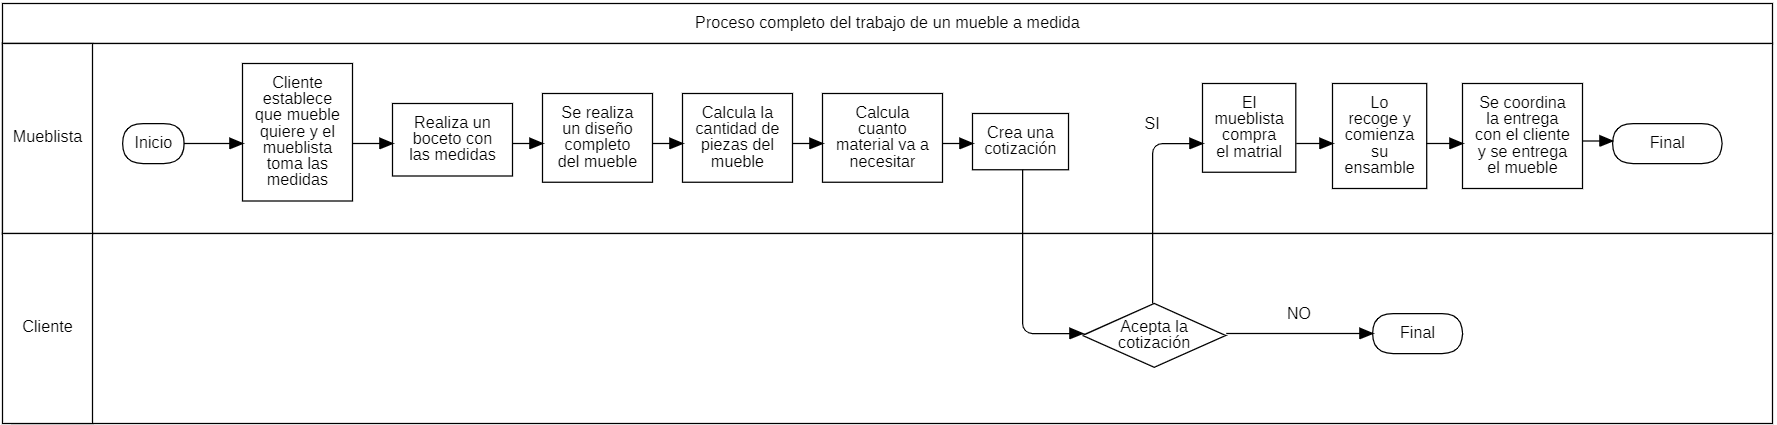
\includegraphics[width=1\textwidth]{imagenes/Diagrama formulación.png}
\end{figure}

\noindent Esta información respalda la pertinencia de desarrollar una plataforma digital que permita al mueblista diseñar muebles a medida en un entorno 2D, visualizando en tiempo real el impacto estético y funcional de sus decisiones, permitiendo además generar una cotización ajustada a materiales, dimensiones y acabados seleccionados.\\

\subsection{Planteamiento del problema}
\begingroup
\small
El proceso de fabricación de muebles a medida es generalmente trasmitido de generación en generación. La oportunidad de mejora o modernización es lenta o muy básica, ya que hay mueblistas que trabajan con bocetos en papel, requieren de mucha precisión en las escalas al momento del dibujo, lo que en muchos casos se ve afectado por las limitaciones educativas presentes en zonas rurales ~\cite{uchile_fabricacion}. Si se considera un mueblista con experiencia en la confección de diseños, el tiempo que invierte al ser todo manual puede tomar entre X y Z horas, ya que se debe confeccionar el diseño considerando que posteriormente se debe estimar la cantidad de cortess (segmentos del material a utilizar) que son requeridos según el tamaño de la “plancha” (tamaño original o máximo del material en cuestión), por lo cual para lograr un presupuesto completo al detalle es un proceso que requiere dedicación y exactitud.\\

\noindent En el mercado existen aplicaciones generales y específicas que eventualmente podrían ser adoptadas por los fabricantes de muebles a medida, pero factores como el costo, la curva de aprendizaje o incluso la tradición del rubro, dan cuenta de la ausencia de una solución que se adapte a sus procesos y que no sean ellos los que deban adaptar sus procesos a la aplicación ~\cite{rural}. Además, en general por los tiempos involucrados en los procesos de cotizaciones iniciales muchas veces no se puede competir con las grandes tiendas, que al tener un stock o que solo requieran de la entrega, genera mucha diferencia comparativamente en los tiempos de respuesta ~\cite{consumidor}.

\subsection{Propuesta de solución}
\begingroup
La solución propuesta consiste en el diseño y desarrollo de una plataforma web para el diseño 2D que permita al mueblista mantener su esquema de trabajo tradicional ahora en un entorno digital, aprovechando además de funcionalidades tecnológicas que buscan apoyarlo en dicho proceso, orientada a apoyar y optimizar el tiempo en el rubro del mueblista o carpintero artesanal. Este sistema considera un espacio de diseño de muebles el cual disponga de los elementos comunes del proceso de fabricación de muebles a medida, por ejemplo espacios modulares de cajoneras, espacios de repisas, colgadores, cubiertas, entre otros. Donde el mueblista pueda escoger cada módulo que necesite, simplificando su usabilidad teniendo que sólo definir las dimensiones (alto, ancho y profundidad) del mueble de acuerdo con los requerimientos del usuario, sin necesidad de ensamblar cada pieza de forma individual. Una vez definido el diseño, el sistema debe calcular automáticamente la cantidad de materiales necesarios para su fabricación (por ejemplo, el número de planchas de melamina requeridas) y generar un listado detallado de materiales.\\

A continuación se describen las etapas involucradas en la elaboración de una cotización para la fabricación de un mueble, junto con sus tiempos estimados y propuestas de optimización:

\begin{itemize}
    \item \textbf{Etapa de diseño:} El mueblista realiza un boceto con las medidas de alto, ancho y profundidad del mueble solicitado. Este proceso puede tardar entre 2 a 4 horas, dependiendo de la complejidad del diseño y la cantidad de piezas involucradas. Se propone optimizar esta etapa mediante el uso de la aplicación web, permitiendo realizar el diseño de forma más rápida en el entorno digital. Se espera una reducción del tiempo de diseño de un 25\%, logrando tiempos entre 1 hora y 45 minutos a 3 horas.

    \item \textbf{Etapa de cubicación:} A partir del diseño, se calcula la cantidad de cortes necesarios de material requerido. Este proceso actualmente se realiza de forma manual y puede tardar entre 2 a 8 horas, dependiendo de la cantidad de piezas y cortes. Con la aplicación web, se busca que la cubicación se realice automáticamente al finalizar el diseño, reduciendo este tiempo a solo minutos, lo que representa una mejora de aproximadamente 90\%.

    \item \textbf{Tiempo total de cotización:} Promediando ambas etapas, el tiempo para entregar una cotización es de aproximadamente 9 horas (3 horas en diseño + 6 horas en cubicación). Con la implementación de la solución propuesta, este tiempo se reduciría significativamente, permitiendo entregar cotizaciones en menos de 4 horas.

    \item \textbf{Impacto en el proceso completo:} Considerando que la fabricación de un mueble puede tardar entre 2 a 10 días, la optimización de las etapas de diseño y cubicación permitiría una mejora promedio del proceso un 15\%.
\end{itemize}

Además se busca contar con una base de datos del historial de muebles para que el mueblista, al momento del diseño, pueda escoger un mueble ya fabricado y modificar las medidas del mueble en general o modificar los módulos según corresponda.\\

Una vez realizado el cálculo de material, se es posible modificar los detalles de la cotización para que el cliente vea el cambio del valor total dependiendo del color, grosor o composición del material.

A su vez la aplicación considera la implementación de un módulo de estadística básica que permitirá registrar y visualizar los periodos del año con mayor demanda de muebles. Este módulo ofrecerá indicadores como el máximo, promedio y mínimo de ventas, segmentados por mes o por año.


\section{Objetivos}
\begingroup
\subsection{Objetivo General}

Optimizar el proceso de diseño y cubicación en la fabricación de muebles a medida, mediante el desarrollo de una aplicación web intuitiva que sirva como herramienta para la creación de diseños personalizados, el cálculo de materiales y la generación de cotizaciones precisas.\\

\subsection{Objetivos específicos}
\begin{enumerate}
\item Implementar una aplicación web que provea de un espacio de diseño en dos dimensiones (2D) orientado a muebles para que el fabricante pueda generar diseños personalizados en base a los requisitos del cliente.

\item Implementar el módulo de cubicación que apoye al fabricante en el cálculo de materiales y costos, agilizando el proceso de propuesta para el cliente. 

\item Desarrollar un respositorio de muebles que permita guardar, reutilizar y modificar diseños previamente realizados.

\item Implementar una biblioteca de materiales, colores, grosores y accesorios que permita y facilite la personalización de los diseños.

\item Automatizar la generación y envío de cotizaciones detalladas e interactivas para que el cliente o mueblista elija entre un abanico de posibilidades.

\item Reducir el tiempo en el proceso de fabricación de muebles a medida en un 15\% respecto al método manual.  

\item Implementar un módulo de estadísticas que permita al mueblista visualizar datos relacionados a demanda e ingresos.

\item Evaluar la satisfacción y usabilidad de la aplicación a través de una encuesta de funcionalidad y usabilidad.
\end{enumerate}
\endgroup

\section{Alcances}
\begingroup
\small
\begin{itemize}
\item La plataforma se diseña para ser utilizada en entorno web responsive.

\item No se considera la implemetación de una aplicación nativa móvil debido a que nativa móvil, debido a que módulos como el de cotizaciones para generar el presupuesto está más pensado para trabajarse en un computador antes que en un teléfono.

\item Los requerimientos se capturan a partir de entrevistas con un mueblista artesanal de la localidad de Teno.

\item La plataforma no considera el diseño de muebles en 3D dado  que se busca que el mueblista mantenga su esquema de trabajo tradicional, sin agregar complejidad al trabajo en pantallas reducidas.

\item Se considera la implementación de un área de diseño 2D especializada para muebles modulares.

\item La plataforma no considera envíos físicos de materiales ni coordinación de logística de entrega.

\item La aplicación no considera gestión de clientes, debido a que está solo orientada a un tipo de usuario.

\item Requerirá que los usuarios tengan conexión a Internet para acceder a la plataforma.

\item La plataforma no considera la implementación de métodos de pagos ni gestión de transacciones financieras.

\end{itemize}
\endgroup



\section{Plan de Trabajo}
\begingroup
\small
 A continuación se presenta el plan de trabajo del proyecto.
\subsection{Descripción de etapas del proyecto}

En esta sección se presentan las etapas del proyecto, tareas más importantes y la cantidad de semanas de duración que se considera realizar en cada etapa.
\begin{enumerate}
\item Requerimientos (1 semana)
    \begin{itemize}
        \item Capturar requerimientos mediante entrevistas.
    \end{itemize}

\item Planificación (2 semanas)
\begin{itemize}
    \item Creación y estimación de historias de usuario.
    \item Definición de tecnologías.
    \item Diseño de modelo de base de datos, mockups y arquitecturas.
\end{itemize}
    
\item Implementación (19 semanas)
\begin{itemize}
    \item Configuración inicial de proyecto.
    \item Implementar módulo de diseño de muebles.
    \item Implementar módulo de visualización de cortes.
    \item Implementar módulo de gestión de cotización.
    \item Implementar módulo de muebles realizados.
    \item Implementar módulo de biblioteca de materiales.
    \item Integración de los módulos desarrollados.
   \item  Implementar módulo estadística.
\end{itemize}

    
\item Evaluación (2 semanas):
\begin{itemize}
    \item Aplicar pruebas de caja negra.
    \item Correcciones de aplicación.
    \item Aplicar prueba de usabilidad con su encuesta.
\end{itemize}

 \item Conclusión (2 semanas):
 \begin{itemize}
    \item Comparar métricas de entrevista inicial y final.
    \item Realizar conclusiones y completar documento.
 \end{itemize}

\end{enumerate}
Se estima un total de 26 semanas para el desarrollo del proyecto dejando una semana para una revisión exhaustiva del documento, además de ir trabajando en la implementación iteración a iteración. Para mayor detalle de la planificación ver la carta Gantt en el anexo A.

\subsection{Tareas para objetivos específicos}
Para cumplir los objetivos específicos se tiene en cuenta las siguientes
 acciones para cada uno de ellos:

\begin{itemize}
\item OE1: Implementar una aplicación web que provea de un espacio de diseño en dos dimensiones (2D) orientado a muebles para que el fabricante pueda generar diseños
personalizados en base a los requisitos del cliente
\begin{enumerate}
\item Etapa 3: Implementar módulo de diseño de muebles.
\item  Etapa 3: Implementar módulo de gestión de cotización.
\end{enumerate}

\item OE2: Implementar el módulo de cubicación que apoye al fabricante en el cálculo de materiales y costos, agilizando el proceso de propuesta para el cliente.
\begin{enumerate}
\item Etapa 3: Implementar módulo de visualización de cortes.
\end{enumerate}

\item OE3: Desarrollar un respositorio de muebles que permita guardar, reutilizar y modificar
diseños previamente realizados.
\begin{enumerate}
\item Etapa 3: Implementar módulo de muebles realizados.
\end{enumerate}

\item OE4: Implementar una biblioteca de materiales, colores, grosores y accesorios que permita y facilite la personalización de los diseños.
\begin{enumerate}
\item Etapa 3: Implementar módulo de biblioteca de materiales.
\end{enumerate}

\item OE5: Automatizar la generación y envío de cotizaciones detalladas e interactivas para que
el cliente o mueblista elija entre un abanico de posibilidades.
\begin{enumerate}
\item Etapa 3: Implementar módulo gestión de cotizaciones.
\end{enumerate}

\item OE6: Optimizar el tiempo en el proceso de fabricación de muebles a medida en un 15\% respecto al método manual.  
\begin{enumerate}
\item Etapa 3: Implementar módulo de diseño de muebles.
\item Etapa 3: Implementar módulo de visualización de cortes.
\item Etapa 3: Implementar módulo de gestión de cotización.
\item Etapa 3: Implementar módulo de muebles realizados.
\item Etapa 3: Implementar módulo de biblioteca de materiales.
\end{enumerate}

\item OE7: Implementar un módulo de estadísticas que permita al mueblista visualizar datos
relacionados a demanda e ingresos.
\begin{enumerate}
\item Etapa 3: Implementar módulo estadística.
\end{enumerate}

\item OE8: Evaluar la satisfacción y usabilidad de la aplicación a través de una encuesta de
funcionalidad y usabilidad.
\begin{enumerate}
\item Etapa 4: Aplicar pruebas de caja negra.
\item Etapa 4: Aplicar prueba de usabilidad con su encuesta.
\end{enumerate}
\end{itemize}

\section{Resumen del capı́tulo}
En este capítulo se presentó el contexto del proyecto, enfocado en la optimización del proceso de diseño y cálculos de la fabricación de muebles a medida. Además, se definió la problemática principal que está asociada al método manual para la estimación de costos y cubicación. Para lo cual se propone como solución una aplicación web que permita el diseño 2D y los cálculos automáticos, así reduciendo los tiempos de entrega y potenciales errores.\\
En el siguiente capítulo se abordarán coceptos básicos del proyecto como tecnologías a utilizar, estado del arte y metodologías de desarrollo y evaluación


\chapter{Marco Teórico}
Este capítulo está orientado a describir conceptos necesarios para entender el foco del proyecto. Además, se presentan las tecnologías que son parte del proyecto.

\section{Conceptos globales}
\begin{itemize}
    \item Cubicación: es un término fundamental en arquitectura, ingeniería y construcción. Es el proceso técnico de medir y calcular las cantidades de materiales, mano de obra y elementos que se necesitarán para ejecutar un proyecto u obra.\\
    Teniendo como objetivo principal cuantificar el proyecto para elaborar un presupuesto preciso, planificar la compra de materiales y programar los trabajos.

    \item Optimización de Corte: Concepto que a menudo se confunde con la cubicación, este es el proceso algorítmico para determinar la disposición óptima de un conjunto de piezas (cortes) sobre un material estándar (como una plancha de melamina) para minimizar el desperdicio de material.

    \item Módulo de Mueble: Se refiere a una unidad o sección pre-diseñada y estandarizada que forma parte de un mueble más grande (Por ejemplo, un módulo de cajonera, un módulo de repisa).

\end{itemize}

\section{Conceptos de software}

\begin{itemize}
    \item Frontend: Es la capa de la aplicación con la que el usuario interactúa directamente, osea, corresponde a todo lo visual de la aplicación web desde la vista del ususario.

\item Backend: Es la capa lógica que se ejecuta en el servidor, invisible para el usuario. Se encarga de procesar las peticiones del frontend, aplicar la lógica de negocio (ej. calcular la cubicación, guardar diseños) e interactuar con la base de datos.

\item Canvas: Es un elemento de HTML que actúa como un 'lienzo' en blanco, permitiendo dibujar gráficos, animaciones y manipular imágenes de forma dinámica usando JavaScript. Es la tecnología base sobre la cual funciona la librería Konva.js~\cite{konva} para crear el espacio de diseño 2D.

\item Servidor: Es el componente que espera, recibe y procesa las solicitudces que envía el cliente, centralizando el procesamiento de datos y ejecutando los algoritmos o funciones. Además es quien interactua directamente con la base de datos para entregar la respuesta al cliente. 

\item Cliente: Se refiere a la persona que le da uso a aplicación, mediante un dispositivo (teléfono, computador, tablet, entre otros) inicia la comunicación solicitando los servicio o recursos que entrega la aplicación.

\item Petición HTTP: Es el mensaje que el cliente envía al servidor para solicitar una acción específica sobre un servicio o recurso. Además, cada petición incluye un método que indica la intención de la acción, siendo estos los más comunes:
\begin{itemize}
    \item GET: Se usa para solicitar datos.
    \item POST: Se usa para enviar datos nuevos.
    \item PUT: Se usa para actualizar datos existentes.
    \item DELETE: Se usa para eliminar datos.
\end{itemize}
\end{itemize}

\section{Tecnologías}
    \subsection{React}
    Para el frontend que representa la interfaz visual en donde el usuario interactuará con el sistema se evaluaron 3 frameworks: React~\cite{react}, Vue~\cite{vue} y Angular~\cite{angular}.\\
    \begin{itemize}
        \item React~\cite{react} es un framework mantenido por Meta y la comunidad, utilizado para construir interfaces de usuario (UI) interactivas y reutilizables. Su enfoque se basa en el concepto de 'componentes', que son partes o piezas de código encapsuladas e independientes que manejan su propio estado.
        \item Vue~\cite{vue} es un framework que cuenta con un enfoque progresivo, siendo creado y mantenido por la comunidad, destacando por su baja curva de aprendizaje y su sintaxis de plantillas basada en HTML.Su flexibilidad le permite ser un núcleo pequeño al que se le pueden añadir módulos oficiales para enrutamiento y gestión de estado a medida que el proyecto crece.
        \item Angular~\cite{angular} es un framework mantenido por google  y a diferencia de los anteriores que son construidos en Javascrip o compatibles, angular es creado sobre TypeScript. Además, sigue una arquitectura Modelo-Vista-Controlador. Otra gran diferencia es la biblioteca ya que angular es una solución 'Todo en uno' que incluye su propio sitema de enrutamiento.
    \end{itemize}
    
    Por su flexibilidad y compatibilidad, React~\cite{react} ha sido seleccionado como el framework ideal para la implementación de la solución propuesta.

 
\begin{table}[H]
    \centering
    
    % --- La \caption va primero para que aparezca arriba ---
    \caption{Comparativa de frameworks web}
    \label{tab:comparativa_frameworks} % <-- Etiqueta para referenciarla
    
    % --- INICIO DE LA TABLA ---
    % Definimos TODAS las columnas como 'p' (párrafo) con un ancho.
    % Los anchos (3.5cm, 4cm, etc.) se pueden ajustar.
    % La suma total debe ser menor que el ancho de la página.
    \begin{tabular}{|p{3.4cm}|p{3.3cm}|p{3.3cm}|p{3.3cm}|} 
        \hline % Línea horizontal superior
        
        % Encabezados en negrita
        \textbf{Característica} & \textbf{React} & \textbf{Angular} & \textbf{Vue.js} \\
        \hline % Línea de separación
        
        % --- Filas con \hline después de CADA una ---
        Tipo & Biblioteca UI & Framework completo (MVC) & Framework progresivo \\
        \hline
        Curva de Aprendizaje & Media & Alta & Baja \\
        \hline
        Ecosistema & Enorme, requiere bibliotecas de terceros & Integral (todo incluido) & Flexible, núcleo pequeño \\
        \hline
        Integración con Canvas & Excelente. Librerías como react-konva facilitan la integración. & Posible, pero más verboso y complejo de integrar. & Buena integración, similar a React. \\
        \hline
        Soporte y Comunidad & Muy alta (mantenido por Meta) & Alta (mantenido por Google) & Alta (mantenida por la comunidad) \\
        \hline
        Rendimiento (DOM) & Alto (Virtual DOM) & Bueno (DOM Real) & Alto (Virtual DOM) \\
        
        \hline % Línea horizontal inferior
    \end{tabular}
\end{table}
    
    \subsection{MongoDB}

    \begin{itemize}
        \item SQL es el lenguaje estándar utilizado para gestionar y consultar base de datos relacionales. Este modelo de base de datos organiza los datos en tablas compuestas por filas y columnas con un esquema rígido y definido.

        \item NoSQL se refiere a la categoría de gestores de bases de datos que difieren del modelo relacional de SQL. Estos sitemas se diseñaron para ofrecer mayor escalabilidad y un esquema flexible.
    \end{itemize}
    Es por la flexibilidad y escalabilidad de la propuesta es que usar una base de datos NoSQL es la mejor opción. Pero dentro de todas las opciones destacan Firebase~\cite{firebase} y MongoDB~\cite{mongodb}.\\

    \begin{itemize}
        \item Firebase~\cite{firebase} es una plataforma de desarrollo propiedad de Google para el desarrollo de aplicaciones web y móviles. Siendo más que una simple base de datos se considera un Backend-as-a-Service(BaaS) que ofrece un conjunto de herramientas y servicios gestionados en la nube para que el desarrollador pueda centrarse en la experiencia del usuario. 

        \item MongoDB~\cite{mongodb} es un sistema gestor de base de datos NoSQL orientado a documentos. Almacena los documentos flexibles similares a JSON denominados BSON, lo que permite manejar datos semiestructurados de forma natural. Este modelo de esquema flexible es útil para casos de uso donde las estructuras de datos son jerárquicas o que evolucionan con el tiempo, ya que permite guardar la información en una sola entidad en lugar de dividirla en múltiples tablas.
    \end{itemize}
    Es por esta flexibilidad, experiencia y forma de manipular documentos, en el esquema que permite guardar, reutilizar y modificar diseños más eficiente y escalable que intentar normalizar esa información en múltiples tablas relacionales, es que MongoDB~\cite{mongodb} es la mejor opción para este proyecto.

\begin{table}[H]
    \centering
    % --- La \caption va primero para que aparezca arriba ---
    \caption{Comparativa de gestor de base de datos}
    \label{tab:comparativa_Base_de_datos} % <-- Etiqueta para referenciarla    
    % --- INICIO DE LA TABLA ---
    \begin{tabular}{|p{3.5cm}|p{5cm}|p{5cm}|} 
        \hline % Línea horizontal superior        
        % Encabezados en negrita
        \textbf{Características} & \textbf{MongoDB (NoSQL)} & \textbf{Bases de Datos Relacionales (SQL)}\\
        \hline % Línea de separación
        
        % --- Filas con \hline después de CADA una ---

Modelo de Datos & Orientado a Documentos.& Orientado a Tablas.\\
\hline
Esquema & Flexible. Cada documento puede tener una estructura única. & Rígido. Todas las filas de una tabla deben seguir la misma estructura.\\
\hline
Manejo de Datos & Natural. Un diseño de mueble completo (con sus módulos, piezas y materiales) puede guardarse en un único documento, preservando su estructura compleja. & Complejo. Requeriría múltiples tablas (ej: Muebles, Modulos, Piezas, Materiales) y consultas complejas para 'reconstruir' un solo diseño.\\
\hline
Aplicable & Proyectos con datos no estructurados o semi-estructurados. & Proyectos con datos altamente estructurados.\\        
        \hline % Línea horizontal inferior
    \end{tabular}
\end{table}

    \subsection{Konva.js}
    Es una librería de Javascript que extiende las capacidades del 'Canvas' 2D de HTML. Permitiendo crear gráficos 2D interactivos y de alto rendimiento, trabajando con las formas (rectángulos, círculos, etc.) como 'objetos' en un 'escenario' (Stage) y 'capas' (Layers). Facilitando la gestión de eventos (arrastrar, soltar), animaciones y transformaciones de objetos.\\
    Es por estos motivos que Konva.js~\cite{konva} es de las mejores opciones para usar en comparación de Fabric.js que fue otra opción a utilizar.

\begin{table}[H]
    \centering    
    % --- La \caption va primero para que aparezca arriba ---
    \caption{Comparativa de librerías para el diseño en lienzo}
    \label{tab:comparativa_librería} % <-- Etiqueta para referenciarla   
    % --- INICIO DE LA TABLA ---
    \begin{tabular}{|p{3.5cm}|p{5cm}|p{5cm}|} 
        \hline % Línea horizontal superior        
        % Encabezados en negrita
        \textbf{Características} & \textbf{Konva.js} & \textbf{Fabric.js}\\
        \hline % Línea de separación        
        % --- Filas con \hline después de CADA una ---
        Enfoque Principal & Lienzo 2D de alto rendimiento con capas (escenario, capas, formas). & Editor de gráficos 2D interactivo y manipulación de objetos. \\
        \hline
        Rendimiento & Optimizado para animaciones y miles de formas. & Bueno, pero puede ser más pesado al manejar muchos objetos.\\
        \hline
        Modelo de Capas & Explícito (Arquitectura de Stage - Layer - Shape). & Basado en un lienzo (canvas) con una colección de objetos. \\
        \hline
        Compatibilidad con React & Excelente. Tiene un wrapper dedicado (react-konva) muy popular. & Buena, pero la integración es más manual. \\
        \hline
        Manejo de Eventos & Robusto y granular (eventos por forma, capa y escenario). & Robusto, centrado en la manipulación de objetos (redimensionar, rotar). \\        
        \hline % Línea horizontal inferior
    \end{tabular}
\end{table}
\subsection{Trello}
Trello es una aplicación de propiedad de Atlassian que se utiliza en la gestión de proyectos visual y colaborativa. Su interfaz se basa en el método Kanban, empleado en tableros, listas y tarjetas para organizar tareas y flujos de trabajo.\\
En comparación a otras herramientas similares como Jira o Asana, Trello presenta una mejor curva de aprendizaje, por lo que esta es la alternativa seleccionada.

\subsection{Email.js}
Entre las herramientas para el envío de correo automatizado destacan principalmente 2 que son Email.js y Sengrid, los cuales describiremos a continuación:
\begin{itemize}
    \item Email.js es un servicio de plataforma que permite enviar correos electrónicos directamente desde las aplicaciones sin necesidad de configurar o mantener un servidor propio. Su funcionamiento se basa en actuar de intermediario seguro. En donde el desarrollador crea plantillas predefinidas dentro del servicio de Email.js

    \item Sengrid es una plataforma de comunicación como servicio basada en la nube, diseñada para la entrega de correos a gran escala. Esta plataforma gestiona una compleja infraesctrucctura de envío, la reputación de las direcciones IP y la escalabilidad, con el objetivo de maximizar la tasa de entrega evitando que estos correos sean marcados como spam.

    Por simplicidad y funcionalidades del plan gratuito, se selecciona Email.js ya que da 2 template y 200 correos mensuales en el plan gratis para usar con cualquier cuenta de correo y viendo las dimesiones y requisitos del proyecto no veo que se requiera más.
    
\end{itemize}

\subsection{Node.js}
Dentro del entrono del backen de la propuesta tenemos muchas opciones para que trabajen la lógica y las interaciones que ocurren destrás de la interfaz del usuario. Entre las opciones tenemos Node.js~\cite{nodejs} con JavaScript, Spring Boot con Java, Laravel con PHP, Flask con python, entre otros. Estas tecnologías permiten relizar las mismas funciones, pero lo que hace la diferencia es la sintaxis de cada lenguaje.\\
Teniendo en cuenta lo anterior y que la propuesta se basa en trabajar con JavaScript la mejor elección es Node.js~\cite{nodejs} con Express por su compatibilidad con la propuesta.

\subsection{Docker}
Docker~\cite{docker} es una plataforma que ofrece el servicio de contendores para desarrolladores mediante imágenes de software para poder construir un programa en un espacio controlado y poder traspasarlo a otro dispositivo sin correr con errores de versiones en las instalaciones que suelen dar problemas. Es por eso que se utiliza Docker al ser un contenedor se puede crear un progama con sus versiones correspondientes y compartirlo sin correr riegos de que pueda fallar.

\subsection{Gloogle Cloud}
Es una plataforma que ofrece servicios en la nube para desarrollar y alojar aplicaciones. Entre sus servicios destacan el alojamiento web, bases de datos, almacenamiento y análisis de datos.\\

\section{Estado del arte}
En cuanto al estado del arte del proyecto, existen distintos tipos de herramientas tanto de pago como gratuitas, a continuación, se mencionan y decriben algunas herramientas reconocidas que estan relacionadas con el proyecto.\\

\noindent 1. \textbf{AutoCAD} ~\cite{AutoCAD}.  Es un software de diseño de paga que se utiliza para dibujar, diseñar y modelar en 2D y 3D de forma precisa con sólidos, superficies, objetos de malla, características de documentación, etc. Incluye características para automatizar tareas y aumentar la productividad, como la comparación de dibujos, el recuento, la adición de objetos y la creación de tablas.\\

\noindent 2. \textbf{IKEA PLanner} ~\cite{IKEA}. Es un software web de IKEA que se encarga de dar ideas según el catálogo de IKEA, en donde se tiene un plano 3D de un espacio genérico de cocina, baño, etc. el cual permite agregar muebles de IKEA para ajustarlo según las necesidades del cliente. \\

\noindent 3. \textbf{Cabinet Vision} ~\cite{Cabinet_Vision}. Es un software de HEXAGON el cual se utiliza para el diseño de muebles 2D y 3D incluyendo el 'listado de cortes', automatizando la exportación a diferentes formatos para las solicitudes de material. Esta aplicación solo es de uso empresarial.\\

\noindent 4. \textbf{Moblo} ~\cite{Moblo}. Es un software que se utiliza para crear diseños 3D de un mueble según las necesidades a partir de figuras simples, permitiendo modificar su color o tipo de material, de uso gratuito. \\

\noindent 5. \textbf{Cut list} ~\cite{CutList}. Es un software que se utiliza para cubicar la lista de cortes de los muebles en la plancha de manera visual y así saber cuanto material se va a usar en el ensamble del mueble. Se ingresan todos los valores de manera manual y también lo que se pierde por corte. Además permite exportar lo listado en PDF o PNG.\\ 

\noindent 6. \textbf{SketchUp} ~\cite{SketchUp}. Es un software que se utiliza para modelado 2D y 3D de estructuras, ya sea cons\-trucción, muebles o diseño de interiores, siendo de paga para profesionales, con posibilidad de vista en realidad virtual (VR).\\

\noindent 7. \textbf{Opticutter} ~\cite{Opticutter}. Es un software web que se usa de calculadora de hoja de corte en línea la cual obtiene una solución utilizando el algoritmo de optimización adecuado. 
\endgroup

\begin{table}[H]
    \centering
    % --- La \caption va primero para que aparezca arriba ---
    \caption{Comparativa de software mencionado}
    \label{tab:comparativa_software} 
    
    % --- INICIO DE LA TABLA ---
    \begin{tabular}{|p{2.2cm}|p{2cm}|p{1cm}|p{1cm}|p{1cm}|p{1cm}|p{1cm}|p{1cm}|p{1cm}|} 
        \hline % Línea horizontal superior
        
        % Encabezados en negrita
        \textbf{Función} & \textbf{Propuesta} & \textbf{1}  & \textbf{2} & \textbf{3} & \textbf{4} & \textbf{5} & \textbf{6} & \textbf{7}\\
        \hline % Línea de separación
        
        % --- Filas con \hline después de CADA una ---
       Diseño 2D/3D & 2D & 2D y 3D & 3D & 2D y 3D & 3D & No & Sí & No\\
       \hline
       Cubicación Automática & Sí & No & No & Sí & Sí & Sí & No & Sí\\
       \hline
       Generación Cotización & Sí & No & No & No & No & No & No & No\\ 
       \hline
       Curva de Aprendizaje & Baja & Alta & Baja & Alta & Media & Baja & Alta & Baja\\
       \hline
       Accesibilidad  & Web  & Nativa & Web & Nativa & Nativa & Web & Nativa & Web\\
        
        \hline % Línea horizontal inferior
    \end{tabular}
\end{table}


\section{Metodologías}
\subsection{Metodologı́a de desarrollo}
Dado que este proyecto será desarrollado de manera individual, se realiza una comparación entre diferentes metodologías ágiles destacando tres opciones: Kanban~\cite{kanban}, Personal Extreme Programming (PXP)~\cite{PXP} y Lean Startup~\cite{lean}, todas son independientes del lenguaje de programación o framework seleccionado. Estas metodologías comparten el enfoque ágil.\\

\noindent \textbf{Personal Extreme Programming (PXP)}: Adaptación individual de la metodología Extreme Programming (XP). PXP usa prácticas como desarrollo incremental, pruebas automatizadas, diseño simple y refactorización continua, pero ajustadas a un entorno unipersonal.\\

\begin{table}[H]
    \centering
    % --- La \caption va primero para que aparezca arriba ---
    \caption{Comparativa de metodologías de desarrollo}
    \label{tab:comparativa_metodologías_de_desarrollo} 
    
    % --- INICIO DE LA TABLA ---
    \begin{tabular}{|p{3cm}|p{3.5cm}|p{3.5cm}|p{3.5cm}|} 
        \hline % Línea horizontal superior
        
        % Encabezados en negrita
        \textbf{Característica} & \textbf{PXP} & \textbf{Kanban}  & \textbf{Lean Startup}\\
        \hline % Línea de separación
        
        % --- Filas con \hline después de CADA una ---
Enfoque Principal & Calidad del código y desarrollo incremental para un solo desarrollador. & Flujo de trabajo visual y continuo. & Validación de hipótesis de mercado/producto.\\
\hline
Funcionamiento &  Basado en prácticas de ingeniería. & Basado en un tablero (Lista 'To Do'). & Se basa en un ciclo de feedback con el cliente/mercado.\\
\hline
Flexibilidad & Alta. Los cambios se gestionan en iteraciones cortas. & Alta. Los cambios pueden entrar al flujo en cualquier momento. & Muy Alta. El objetivo es cambiar basado en los datos aprendidos.\\
\hline
Disciplina Técnica & Alta. Exige prácticas de ingeniería de software. & Baja. No se enfoca en prácticas de código, solo de flujo. & Baja. El foco no es la calidad técnica, sino la velocidad para aprender.\\
\hline
Aplicabilidad & Alta. Se enfoca en la ejecución de un proyecto con requisitos definidos y alta calidad técnica. & Alta. Útil para gestionar tareas, pero no guía la calidad del software. & Medio. Prioriza   validar un producto en el mercado.\\
        
        \hline % Línea horizontal inferior
    \end{tabular}
\end{table}

\noindent Para este proyecto se elige Personal Extreme Programming (PXP) dado que se adapta a las características requeridas en el contexto. Además PXP se centra en la calidad del código desde el inicio, además de que permite avanzar en ciclos cortos, lo que facilita ajustes constantes y mejora continua proporcionando flexibilidad durante el desarrollo.\\

\noindent Para el desarrollo de esta propuesta se seguirán distintas fases que contempla la metodología:\\

\noindent \textbf{Requerimientos}: Durante esta etapa se captan los requisitos del proyecto en conjunto con el cliente. Estos requerimientos se convierten en la fase siguiente en historias de usuario, que permiten enfocar el desarrollo en la experiencia del usuario.\\

\noindent \textbf{Planificación}: Durante esta fase se desarrolla la creación y estimación de las historias de usuarios, la elección de tecnologías a utilizar, diseño de mockups y arquitectura.\\

\noindent \textbf{Iteración}: Durante esta etapa se indica la inicialización de cada iteración o ciclo, la cual puede durar entre 1 y 4 semanas.\\

\noindent \textbf{Diseño}: Durante esta fase se desarrolla el diseño lógico de módulos y funciones correspondientes a cada iteración.\\ 

\noindent \textbf{Implementación}: Durante esta fase se realiza el desarrollo mediante programación de las historias de usuario asociadas a una tarea, para salir de esta fase debe funcionar sin errores y pasar todas las pruebas unitarias, en caso de no ser así se debe refactorizar el código realizado.\\

\noindent \textbf{Sistema de Pruebas}: Durante esta fase se realiza el testeo para validar las funcionalidades desarrolladas durante la iteración y se debe verificar si la solución implementada con los requisitos iniciales del proyecto.\\

\noindent \textbf{Retrospectiva}: Esta fase demarca el final de cada iteración, se realiza un análisis de los datos recopilados durante las fases y de las propuestas de mejora. Esta etapa puede marcar el inicio de una nueva iteración o el final del desarrollo del proyecto.\\

\begin{figure}[H]
    \centering
    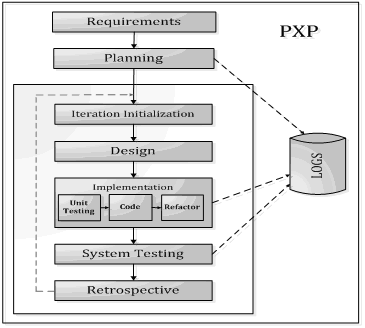
\includegraphics[width=0.5\textwidth]{imagenes/PXP-process-phases.png}
    \caption{Diagrama de las fases de metodología Personal Extreme Programming (PXP) }
    \label{fig: diagrama}
\end{figure}
\subsection{Metodología de evaluación}
    \subsubsection{ Prueba de caja negra}
Las pruebas de caja negra se centran en evaluar el comportamiento funcional de la aplicación desde la perspectiva del usuario, sin considerar la estructura interna del código ni los algoritmos utilizados. Este enfoque permite validar que el sistema responde correctamente a los datos de entrada y cumple con los requisitos establecidos en la documentación técnica. Para ello, se diseñan casos de prueba basados en las especificaciones funcionales, verificando que las salidas obtenidas coincidan con las esperadas.~\cite{caja_negra}
\begin{figure}[H]
    \centering
    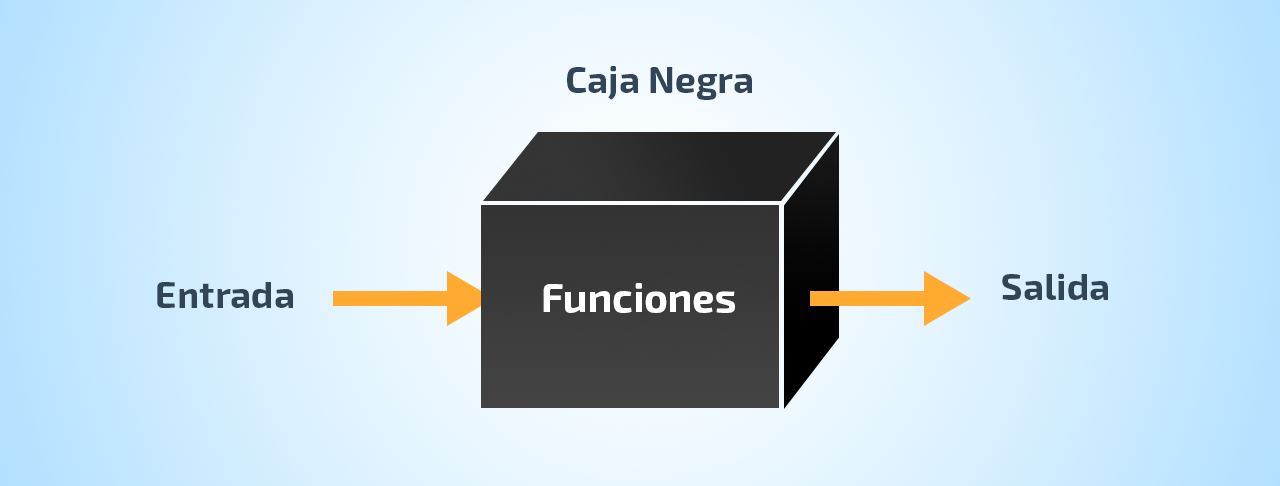
\includegraphics[width=0.6\textwidth]{imagenes/caja_negra.png}
    \caption{Proceso de Prueba de Caja Negra}
    \label{fig: diagrama}
\end{figure}
\subsubsection{Prueba de usabilidad}
Las pruebas de usabilidad permiten validar la experiencia del usuario final con la aplicación desarrollada. Para este propósito, se aplicará la técnica System Usability Scale (SUS), una herramienta creada por John Brooke en 1986 y ampliamente utilizada en la industria del software. Esta prueba consiste en un cuestionario de 10 afirmaciones evaluadas mediante la Escala de Likert, donde los participantes expresan su nivel de acuerdo. A partir de estas respuestas, se calcula un puntaje total entre 0 y 100 que refleja la percepción de usabilidad: valores inferiores a 50 indican una experiencia inaceptable, entre 50 y 68 se consideran deficientes o mediocres, y puntuaciones superiores a 68 reflejan una aceptación adecuada del sistema por parte del usuario.~\cite{SUS}


\section{Resumen del capı́tulo}
En este capítulo se describieron los conceptos necesarios para entender el proyecto, además se describieron las tecnologías a utilizar, comparando opciones y justificando las elecciones. También se abordó el estado del arte, en donde se presentaron aplicaciones que ofrecen funcionalidades similares a la propuesta. Finalmente se detalló la métodología de desarrollo y evaluación, justificando sus elecciones.\\
En el siguiente capítulo se abordará la aplicación de la metodología elegida, junto a las adaptaciones necesarias para el proyecto y los resultados esperados de los objetivos específicos.


\chapter{Metodologías}
En este capítulo se presentan describe como la metodología de desarrollo ya presentada se aplicará en la propuesta y los resultados esperados de los objetivos específicos. 
\begingroup
\section{Personal Extreme Programming (PXP)}
Como se mencionó en el capítulo anterior, PXP al ser la versión individual de Extreme Progamming (XP), se basa en el desarrollo personal de software manteniendo las fases claves como Requerimientos, Planificación, Iteración y Pruebas. 

\subsection{Requerimientos}
Durante esta etapa donde el desarrollador realiza una entrevista con al cliente, para visualizar lo requerimientos del sistema. Estos requerimientos se convierten en la fase siguiente en historias de usuario, que permiten enfocar el desarrollo en la experiencia del usuario.

\subsection{Planificación}
Durante esta etapa la actividad central consiste en la creación, priorización y organización de las historias de usuario (HU). También se toman las decisiones de la composición de la aplicación, tales como las configuraciones de las tecnologías a utilizar, arquitecturas de software y mockups.\\
\begin{table}[H]
    \centering
    % --- La \caption va primero para que aparezca arriba ---
    \caption{Clasificación de las historias de usuario}
    \label{tab:Clasificación_historias_de_usuario} 
    
    % --- INICIO DE LA TABLA ---
    \begin{tabular}{|p{1,5cm}|p{2cm}|p{11cm}|} 
        \hline % Línea horizontal superior
        
        % Encabezados en negrita
        \textbf{HU} & \textbf{Actor} & \textbf{Descripción}\\
        \hline % Línea de separación
        
        % --- Filas con \hline después de CADA una ---
HU01 & Mueblista & Como usuario quiero iniciar sesión en el sistema.\\
\hline
HU02 & Mueblista & Como ususario quiero un canvas 2D para poder hacer diseños. \\
\hline
HU03 & Mueblista & Como usuario quiero crear, guardar, cargar y eliminar el diseño de un mueble.\\
\hline
HU04 & Mueblista & Como usuario quiero que el diseño se pueda hacer módular.\\
\hline
HU05 & Mueblista & Como usuario quiero que las medidas de los módulos agregados puedan ser editables.\\
\hline
HU06 & Mueblista & Como usuario quiero que los módulos sean móviles para acomodarlos según la necesidad.\\
\hline
HU07 & Mueblista & Como usuario quiero que el sistema me calcule la cantidad de material.\\
\hline
HU08 & Mueblista & Como usuario quiero que se muestre un listado de las piezas que se van a utilizar.\\
\hline
HU09 & Mueblista & Como usuario quiero que el sistema pueda generar cotizaciones a partir del diseño.\\
\hline
HU10 & Mueblista & Como usuario quiero que se vea una previsualización de la cotización.\\
\hline
HU11 & Mueblista & Como usuario quiero que en la previsualización de la cotización se puedan personalizar.\\
\hline
HU12 & Mueblista & Como usuario quiero que las cotizaciones se puedan exportar como pdf\\
\hline
HU13 & Mueblista & Como usario quiero que el sistema permita enviar cotizaciones por correo\\
\hline
HU14 & Mueblista & Como usuario quiero disponer de una biblioteca de materiales\\
\hline
HU15 & Mueblista & Como ususario quiero poder agregar, editar y eliminar materiales de la biblioteca\\
\hline
HU16 & Mueblista & Como usuario quiero ver estadíscas básicas \\
\hline
HU17 & Mueblista & Como usuario quiero que se puedan filtrar las estadísticas por periodos\\
        \hline % Línea horizontal inferior
    \end{tabular}
\end{table}
\vspace{2em}
Para la clasificación de prioridad se utilizará la clasificación MuSCoW la cual es un una técnica utilizada en la priorización de requerimientos en el desarrollo de software. MuSCoW es eln acrónimo derivado de Must have (Debe tener), Should have (Debería tener), Could have (Podría tener) y Won't have (No tendrá, por ahora).A continuación se describen las categorías:
\begin{itemize}
    \item Must Have: Representa los objetivos esenciales o imprescindibles para que el sistema funcione correctamente. sin estos elementos, el producto final sería inviable y no cumpliría con su propósito.

    \item Should Have: Estos son lo requisitos importantes, pero no fundamentales para el funcionamiento del sistema. Si bien su ausencia no generará errores críticos, pero su implementación mejora la funcionalida del sistema y se considera de alta prioridad en caso de que el tiempo y los recursos estén a favor.

    \item Could Have:  Incluyen características adicionales que mejorarían la experiencia del usuario o la eficiencia del sistema. Se implementan solo si hay tiempo y recursos suficientes tras completar los requisitos de mayor prioridad.

    \item Won't have: Requisitos que se han identificado como no esenciales en esta etapa del esarrollo. No se implementarán en la versión actual del proyecto, aunque podrían considerarse en futuras versiones o iteraciones del sistema.
\end{itemize}

Para poder calcular el peso a las historias de ususario utilizaré la secuencia de Fibonacci ya que es una técnica de estimación del esfuerzo requerido para cada historia de usuario. El uso de esta escala no lineal obliga a diferenciar claramente entre tareas, evitando la falsa precisión de las estimaciones temporales en etapas tempranas del desarrollo. En esta escala permite categorizar las tareas de la siguiente manera:

\begin{itemize}
    \item Baja complejidad (1-3 pts.): Tareas rutinarias, de bajo riesgo y con requisitos claros.

    \item Media Complejidad (5 pts.): Tareas que requieren lógica específica o integración de componentes.

    \item Alta Complejidad (8-13 pts.): Tareas con alta incertidumbre tecnológica, lógica algorítmica compleja o dependencias críticas.
\end{itemize}


A continuación, se presenta la clasificación MuSCoW para la prioridad de desarrollo y estimación de esfuerzo de las historias de usuario:
\begin{table}[H]
    \centering
    % --- La \caption va primero para que aparezca arriba ---
    \caption{Clasificación MuSCoW y estimación de esfuerzo de las historias de usuario}
    \label{tab:Clasificación_historias_de_usuario} 
    
    % --- INICIO DE LA TABLA ---
    \begin{tabular}{|p{2cm}|p{2cm}|p{3cm}|} 
        \hline % Línea horizontal superior
        
        % Encabezados en negrita
        \textbf{HU} & \textbf{MuSCoW} & \textbf{Estimación de esfuerzo}\\
        \hline % Línea de separación
        
        % --- Filas con \hline después de CADA una ---
HU01 & Must & 3\\
\hline
HU02  & Must & 5\\
\hline
HU03 & Must & 3\\
\hline
HU04 & Must & 8\\
\hline
HU05 & Must & 3\\
\hline
HU06 & Must & 3\\
\hline
HU07 & Must & 13\\
\hline
HU08 & Must & 3\\
\hline
HU09 & Should & 5\\
\hline
HU10 & Should & 2\\
\hline
HU11 & Could & 5\\
\hline
HU12 & Should & 2\\
\hline
HU13 & Won't & 3\\
\hline
HU14 & Should & 2\\
\hline
HU15 & Should & 3 \\
\hline
HU16 & Could & 5 \\
\hline
HU17 & Could & 2\\
        \hline % Línea horizontal inferior
    \end{tabular}
\end{table}

\begin{table}[H]
    \centering
    % --- La \caption va primero para que aparezca arriba ---
    \caption{Objetivos específicos con sus historias de usuario}
    \label{tab:OE_historias_de_usuario} 
    
    % --- INICIO DE LA TABLA ---
    \begin{tabular}{|p{7cm}|p{7cm}|} 
        \hline % Línea horizontal superior
        
        % Encabezados en negrita
        \textbf{Objetivos Específicos (resumidos) } & \textbf{Historias de Usuario (HU)}\\
        \hline % Línea de separación
        
        % --- Filas con \hline después de CADA una ---
OE01: Implementar canvas 2D & HU02, HU04, HU05, HU06\\
\hline
OE02: Implementar el módulo de cubicación & HU07, HU08\\
\hline
OE03: Gestionar diseños realizados & HU03\\
\hline
OE04: Biblioteca de materiales & HU14, HU15\\
\hline
OE05: Automatizar cotizaciones & HU09, HU10, HU12, HU11, HU13\\
\hline
OE06: Reducir el tiempo del proceso de fabricación de muebles & Este objetivo es el resultado de OE01, OE02 y OE05. Se logra principalmente con HU02, HU04, HU07, HU09.\\
\hline
OE07: Implementar estadísticas & HU16, HU17\\
\hline
OE08: Evaluar la satisfacción y usabilidad & Aplicando encusta SUS sobre las interfaces principalmente en: HU02, HU05, HU09 y HU014\\
\hline
Requisito General & HU01\\
        \hline % Línea horizontal inferior
    \end{tabular}
\end{table}

\subsubsection{Planificación historias de usuario}
\begin{table}[H]
    \centering
    % --- La \caption va primero para que aparezca arriba ---
    \caption{Planificación historias de usuario}
    \label{tab:planificacion_historias_de_usuario} 
    
    % --- INICIO DE LA TABLA ---
    \begin{tabular}{|p{2cm}|p{5cm}|p{7cm}|} 
        \hline % Línea horizontal superior
        
        % Encabezados en negrita
        \textbf{Iteración} & \textbf{Historias de Usuario} & \textbf{Objetivo de la Iteración}\\
        \hline % Línea de separación
        
        % --- Filas con \hline después de CADA una ---
Iteración 1 & HU01 & configuración del stack técnologico e inicio de sesión\\
\hline
Iteración 2 &  HU02, HU03, HU04, HU05, HU06 & Construir el diseñador 2D modular (guardar y cargar).\\
\hline
Iteración 3 & HU07, HU08 & Implementar el algoritmo de cubicación y mostrar la lista de piezas. \\
\hline
Iteración 4 & HU09, HU10, HU12, HU14, HU15 & Generar cotizaciones en PDF y su personalización.\\
\hline
Iteración 5 & HU14, HU15 & Gestionar biblioteca de materiales.\\
\hline
Iteración 6 & HU16, HU17 & Implementar estádisticas generales.\\
\hline
Iteración 7 & HU13 & Implementar notificaciones por correo.\\
\hline
Iteración 8 & HU03 & Implementar biblioteca de muebles\\
        \hline % Línea horizontal inferior
    \end{tabular}
\end{table}
\subsection{Iteración}
Esta estapa es la de mayor duración e importancia en la metodología, la cual se divide en las siguientes estapas: Inicio de Iteración, Diseño, Implementación, Sistema de pruebas y Retrospectiva. A continuación, se describe la aplicación de cada una de las etapas.

\subsubsection{Inicio de iteración}
Durante esta etapa se crean las tareas específicas para cada historia de usuario correspondientes a cada iteración. Para llevar el control de las tareas se pueden usar diferentes herramientas mientras permitan una estructura sólida de tabla.
\begin{figure}[H]
  \vspace*{1cm}
  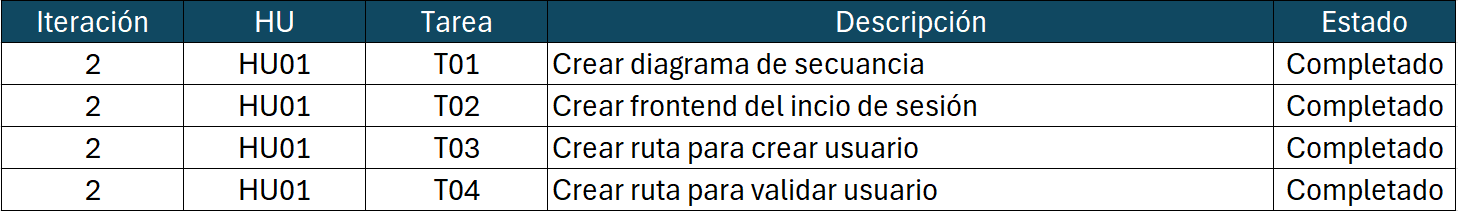
\includegraphics[width=1.1\linewidth]{imagenes/tareas.png}
  \vspace*{1cm}
  \caption{Extracto de la tabla de registro de tareas}
\end{figure}

\subsubsection{Diseño}
En esta etapa, se crean los diagramas de secuencia de las historias de usuario
asociadas a la iteración. A continuación, se muestra la un diagrama de secuencia de la función de login o inicio de sesión.
\begin{figure}[H]
  \vspace*{1cm}
  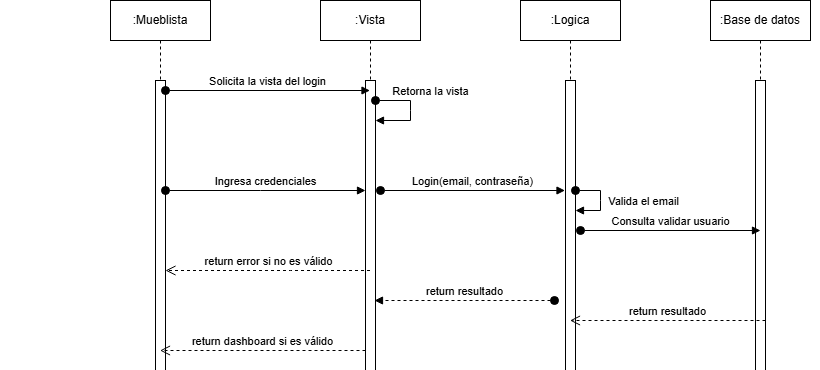
\includegraphics[width=.9\linewidth]{imagenes/secuencia2.drawio.png}
  \vspace*{1cm}
  \caption{Diagrama de secuencia para inicio de sesión}
\end{figure}


\subsubsection{Implementación}
En esta etapa se lleva a cabo el desarrollo de código, pruebas unitarias y refactorización. La implementación sigue los diagramas de secuencia para guiar el flujo de las funcionalidades y los mockups propuestos. Si bien la metodología PXP recomienda el enfoque TDD o Test-Driven Development, que se basa en crear pruebas unitarias, se procede con código y finalmente con la refactorización, pero para este caso se ajustará el proceso a desarrollar el código, proceder con las pruebas unitarias y finalizar con refactorizar en caso de fallar alguna prueba.

\subsubsection{Sistema de Pruebas}
En esta etapa se crean y ejecutan las pruebas correspondientes a todas las tareas
definidas en el Inicio de Iteración. En caso de fallar alguna prueba se debe volver a la fase de implementación para corregir el error, en caso de aprobar las pruebas se procede a la siguiente etapa. Para llevar el control se pueden usar diferentes herramientas que permitan listar para llevar una buena gestión de las pruebas hechas y tareas realizadas.

\begin{figure}[H]
  \vspace*{1cm}
  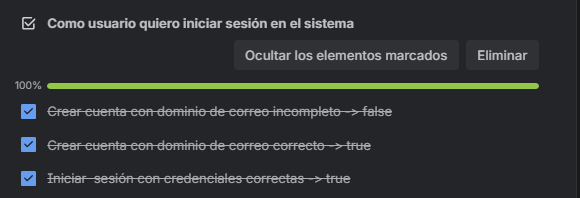
\includegraphics[width=.9\linewidth]{imagenes/iteracio 2.png}
  \vspace*{1cm}
  \caption{Extracto de lista de comprobación}
\end{figure}

\subsubsection{Retrospectiva}
Esta etapa marca el final de la iteración, en donde se deben verificar si el 'peso'
estimado para las historias de usuario es igual al que tomó completarla, para evitar
subestimar o sobreestimar tareas o historias futuras. También permite evaluar el avance de la propuesta, logrando identificar como se van cumpliendo con los plazos e identificar potenciales retrasos o problemas. Al finalizar esta etapa se tiene que decidir si se da inicio a una nueva iteración o finalizar las iteraciones y dar por completado el desarrollo de la aplicación.



\section{Metodologías de evaluación}
 En esta sección se presentan las metodologías de evaluación a utilizar en el proyecto.

\subsection{Prueba de caja negra}
Las pruebas de caja negra es un método de evaluación de software, la cual se enfoca en las entradas y salidas del programa, sin la necesidad de tener conocimiento de la estructura interna del programa.\\
PAra mantener el registro de las pruebas se pueden usar diferentes tipos de herramientas, en donde solo se necesita una estructura que contenga el identificador, la descripción de la prueba, las entradas, las salidas y el resultado esperado. A continuación, en la Figura 3.4 se ilustra una hoja de cálculo que contiene un ejemplo de la estructura de los registros de pruebas. 

\begin{figure}[H]
  \vspace*{1cm}
  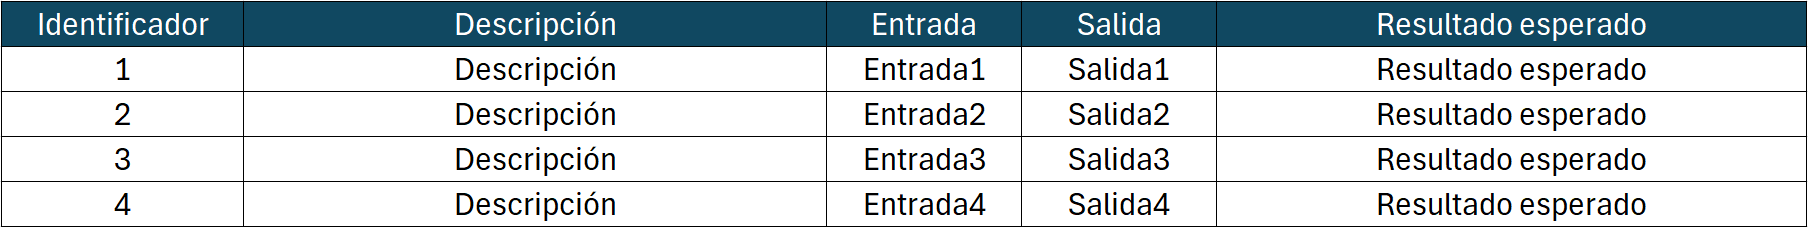
\includegraphics[width=.9\linewidth]{imagenes/Pcajanegra.png}
  \vspace*{1cm}
  \caption{Registro pruebas de caja negra}
\end{figure}
\subsection{Prueba de usabilidad}
La prueba de usabilidad o SUS permite que el usuario evalúe la usabilidad de la aplicación mediante una encuesta, para la cual no se requiere conocimientos de software o de un lenguaje técnico para entender y responder las preguntas. Esta encuesta cuenta con 10 preguntas estándares, que serán respondidas en una escala del 1 al 5, tomando 1 como 'totalmente en desacuerdo', 2 como 'en desacuerdo', 3 como 'Neutro', 4 como 'de acuerdo' y 5 como 'totalmente de acuerdo'. A continuación se detallan las preguntas
\begin{enumerate}

    \item Creo que me gustaría utilizar este sistema con frecuencia
    \item Encontré el sistema innecesariamente complejo
    \item Pensé que el sistema era fácil de usar
    \item Creo que necesitaría el apoyo de un técnico para poder utilizar este sistema
    \item Encontré que las diversas funciones de este sistema estaban bien integradas
    \item Pensé que había demasiada inconsistencia en este sistema
    \item Me imagino que la mayoría de la gente aprendería a utilizar este sistema muy rápidamente
    \item Encontré el sistema muy complicado de usar
    \item Me sentí muy seguro usando el sistema
    \item Necesitaba aprender muchas cosas antes de empezar con este sistema 
\end{enumerate}
Para obtener el grado de aceptación de la aplicación se debe realizar el siguiente cálculo:
\begin{itemize}
    \item Suma las respuestas de los enunciados impares y después resta 5, ejemplo: (2 + 3 + 1 + 5 + 2) = 13 – 5 = 8
    
    \item Suma las respuestas de los enunciados pares y resta ese total a 25, ejemplo: (1 + 2 + 2 + 3 + 1) = 25 – 9 = 16
    
    \item Suma ambos resultados y multiplícalo por 2,5, ejemplo: (8 + 16) * 2,5 = 60
    
\end{itemize}
El puntaje final, oscila entre 0 y 100, permitiendo clasificar la usabilidad de la aplicación como Inaceptable (0-49), Mediocre (50-68) o Aceptable (69-100).
\endgroup

\section{Resultados esperados}
A continuación, se presentan los objetivos específicos con sus resultados esperados, además del medio para comprobarlo
\begin{enumerate}
\item OE1: Implementar una aplicación web que provea de un espacio de diseño en dos dimensiones (2D) orientado a muebles para que el fabricante pueda generar diseños personalizados en base a los requisitos del cliente.
\begin{itemize}
    \item Resultado esperado: Se espera un módulo de diseño funcional e interactivo, que le permita al mueblista arrastrar, soltar y redimensionar los módulos de muebles, logrando representar los requisitos del mueblista.
    \item Pruebas para lograr resultado esperado: Pruebas de caja negra para la funcionalidad del Canvas.
\end{itemize}

\item OE2: Implementar el módulo de cubicación que apoye al fabricante en el cálculo de materiales y costos, agilizando el proceso de propuesta para el cliente. 
\begin{itemize}
    \item Resultado esperado: Un algoritmo de cálculo integrado que procese automáticamente las diemnsiones del diseño 2D y cuente con un listado de piezas y la cantidad de planchas de material necesarias.
    \item Pruebas para lograr resultado esperado: Pruebas de caja negra comparando el resultado del algoritmo y un cálculo manual.
\end{itemize}

\item OE3: Desarrollar un respositorio de muebles que permita guardar, reutilizar y modificar diseños previamente realizados.
\begin{itemize}
    \item Resultado esperado: Un sistema de datos en MongoDB que permita crear, leer, actualizar y eliminar diseños de muebles.
    \item Pruebas para lograr resultado esperado: Pruebas de caja negra para la integración de la base de datos.
\end{itemize}

\item OE4: Implementar una biblioteca de materiales, colores, grosores y accesorios que permita y facilite la personalización de los diseños.
\begin{itemize}
    \item Resultado esperado: Un catálogo digital gestionable en donde el mueblista pueda administrar los atributos de los materiales, los cuales se vinculan dinámicamente al cálculo de costos del diseño.
    \item Pruebas para lograr resultado esperado: Pruebas de caja negra de ingreso y edición de datos.
\end{itemize}

\item OE5: Automatizar la generación y envío de cotizaciones detalladas e interactivas para que el cliente o mueblista elija entre un abanico de posibilidades.
\begin{itemize}
    \item Resultado esperado: La capacidad del sistema para generar un documento formal en formato PDF con los valores correctos de precio y material.
    \item Pruebas para lograr resultado esperado: Pruebas de caja negra revisando los valores del PDF generado.
\end{itemize}

\item OE6: Reducir el tiempo en el proceso de fabricación de muebles a medida en un 15\% respecto al método manual.  
\begin{itemize}
    \item Resultado esperado: Una disminución cuantificable de al menos un 15\% en el tiempo total requerido para completar el ciclo de Diseño + Cubicación + Cotización en comparación con el método tradicional manual.
    \item Pruebas para lograr resultado esperado: Medición de tiempos comparando el flujo manual con el uso de la aplicación en un caso de prueba estándar.
\end{itemize}

\item OE7: Implementar un módulo de estadísticas que permita al mueblista visualizar datos relacionados a demanda e ingresos.
\begin{itemize}
    \item Resultado esperado: Un panel de visualización que presente datos claros sobre la cantidad de proyectos realizados y estimaciones de ingresos, filtrables por periodos de tiempo.
    \item Pruebas para lograr resultado esperado: Pruebas de caja negra con los valores de los gráficos o datos visibles.
\end{itemize}

\item OE8: Evaluar la satisfacción y usabilidad de la aplicación a través de una encuesta de funcionalidad y usabilidad.
\end{enumerate}
\begin{itemize}
    \item Resultado esperado: Obtener una calificación de usabilidad superior a 68 puntos que es un nivel "Aceptable"  en la escala SUS, validando que la interfaz es intuitiva para el perfil del mueblista artesanal.
    \item Pruebas para lograr resultado esperado: Resultados de la encuesta SUS aplicada al usuario final tras las pruebas.
\end{itemize}

\section{Resumen del capı́tulo}
En este capítulo se detalló la forma en que se aplicará la metodología PXP en la propuesta. Además, se abordan las métodologías de evaluación y el funcionamiento de estas como pruebas de software para pruebas de caja negra y pruebas cualitativas para evaluar cuantitativamente con la encuenta SUS. Finalmente se abarcan los resultados esperados de los objetivos específicos.\\
En el siguiente capítulo se abarca la implementación de la metodología PXP, siguiendo sus etapas y explicando que se realizó en cada una.


\chapter{Desarrollo}
El presente capítulo está orientado a presentar la implementación de la metodología en desarrollo.

\section{Análisis de factibilidad}
Como se busca la viabilidad de la propuesta a continuación se presenta el análisis técnico y económico para revisar los recursos y gastos asociados al proyecto obteniendo que tan rentable es la propuesta.

\subsection{Factibilidad técnica}
El análisis de factibilidad técnica evalúa la disponibilidad de recursos de hardware y software necesarios para el desarrollo, implementación y operación del sistema propuesto. Dada la naturaleza de la solución y el perfil del usuario final, este análisis se desglosa en:

1. Requisitos del lado del cliente (Hardware y Software):
A diferencia de software de diseño tradicional como AutoCAD, que exige estaciones de trabajo de alto rendimiento, la solución propuesta traslada la carga de procesamiento al navegador web mediante el uso de estándares HTML5.

Hardware: La aplicación requiere un navegador web moderno con soporte Canvas API (ej. Google Chrome, Mozilla Firefox, Safari o Edge en sus versiones actualizadas). Esto garantiza una alta disponibilidad, ya que estos navegadores son gratuitos y estándar en el mercado.

Recursos de Hardware: La librería seleccionada, Konva.js, realiza el renderizado de gráficos vectoriales en el cliente. Para garantizar una experiencia fluida, se estima un requisito mínimo de 4 GB de memoria RAM y un procesador de gama media o baja. Esto hace viable su uso en computadores portátiles estándar y teléfonos inteligentes no tan actuales, alineándose con la realidad económica de las PYMES objetivo.

2. Conectividad y Latencia en Entornos Rurales Considerando que el despliegue se orienta a zonas como Teno , donde la conexión a internet puede ser inestable o de ancho de banda limitado, la arquitectura de Single Page Application (SPA) implementada con React  es técnicamente la más adecuada.


Justificación: Una vez cargado el bundle inicial de la aplicación, la interacción de diseño (arrastrar, soltar, redimensionar figuras) se ejecuta localmente en el navegador del usuario usando JavaScript, sin necesidad de realizar peticiones al servidor por cada movimiento. Esto minimiza la dependencia de una conexión de alta velocidad constante, requiriendo internet principalmente para el inicio de sesión y el guardado final del diseño, lo cual mitiga los riesgos de desconexión durante el proceso creativo.


3. Madurez y Disponibilidad del Stack Tecnológico El desarrollo se sustenta en el stack MERN (MongoDB, Express, React, Node.js), tecnologías de código abierto con licencias permisivas (MIT), lo que elimina barreras legales y de costos por licenciamiento.

Sostenibilidad: Estas tecnologías cuentan con documentación extensa y comunidades activas, asegurando la mantenibilidad del código a largo plazo.


Portabilidad: El uso de Docker  para la contenerización permite que el sistema sea agnóstico a la infraestructura del servidor, garantizando que la aplicación pueda migrarse entre distintos proveedores de nube (Google Cloud, AWS, o servidores locales) sin conflictos de dependencias ni reescritura de código.

Conclusión Técnica: En base a lo expuesto, el proyecto es técnicamente factible. No requiere hardware especializado por parte del usuario final, se adapta a las condiciones de conectividad de zonas rurales gracias a su arquitectura SPA y utiliza tecnologías estándar de la industria que aseguran su viabilidad operativa y escalabilidad futura.

\subsection{Factibilidad económica}
La factibilidad económica evalúa los costos necesarios para la propuesta.\\
\begin{table}[H]
    \centering
    % --- La \caption va primero para que aparezca arriba ---
    \caption{Factibilidad económica}
    \label{tab:factibilidad_económica} 
    
    % --- INICIO DE LA TABLA ---
    \begin{tabular}{|p{5cm}|p{5cm}|p{2cm}|} 
        \hline % Línea horizontal superior
        
        % Encabezados en negrita
        \textbf{Servicio} & \textbf{Técnología} & \textbf{Costo}\\
        \hline % Línea de separación
        
        % --- Filas con \hline después de CADA una ---
        Frontend & React & \$0\\
        \hline
        Backend & Node.js & \$0\\
        \hline
        Base de datos & MongoDB & \$0\\
        \hline 
        Servicio de correo & Email.js &\$0\\
        \hline
        Control de versiones & GitHub & \$0\\
        \hline
        Contenedor & Docker & \$0\\    
        \hline % Línea horizontal inferior
    \end{tabular}
\end{table}
Teniendo esta tabla de costos 4.1 se obtiene que el gasto de licencias de software es de \$0 pesos chilenos, ya que todas las herramientas tecnológicas que componen esta propuesta son gratuitas o de código abierto por lo que a nivel de gastos esta propuesta es muy viable ya que cuando empiece a escalar y se requiera de planes de pago a mayor escala el mismo proyecto ya lo podrá sustentar.  \\
Teniendo en cuenta el despliegue de la aplicación en un servidor en la nube, se puede considerar el uso de servicios como Google Cloud Platform (GCP), Amazon Web Services (AWS) o Microsoft Azure. Estos servicios ofrecen planes gratuitos con ciertas limitaciones que podrían ser suficientes para un proyecto inicial o de pequeña escala.\\
Pero si se requiere de un plan pago, los costos pueden variar dependiendo del proveedor y los recursos utilizados. Por ejemplo, una instancia básica de propósito general con 2vCPU y 4 GB de RAM en un servidor de Google Cloud puede costar alrededor de \$57 USD, dependiendo de la configuración y el uso.\\


\section{Diseño de software}
Se presentan los elementos claves en el diseño de software, tales como arquitectura física, arquitectura logíca, modelo de datos y mockups principales.
\subsection{Arquitectura fisíca}
La arquitectura física propuesta sigue el modelo cliente-servidor, el cual se ilustra en la figura 4.1 a continuación. En este modelo, el servidor actúa como el núcleo de procesamiento, recibiendo las solicitudes iniciadas por el cliente (frontend), ejecuta la lógica correspondiente en el backend y gestiona las consultas con la base de datos para finalmente retornar la respuesta requerida al usuario.
\begin{figure}[H]
  \vspace*{1cm}
  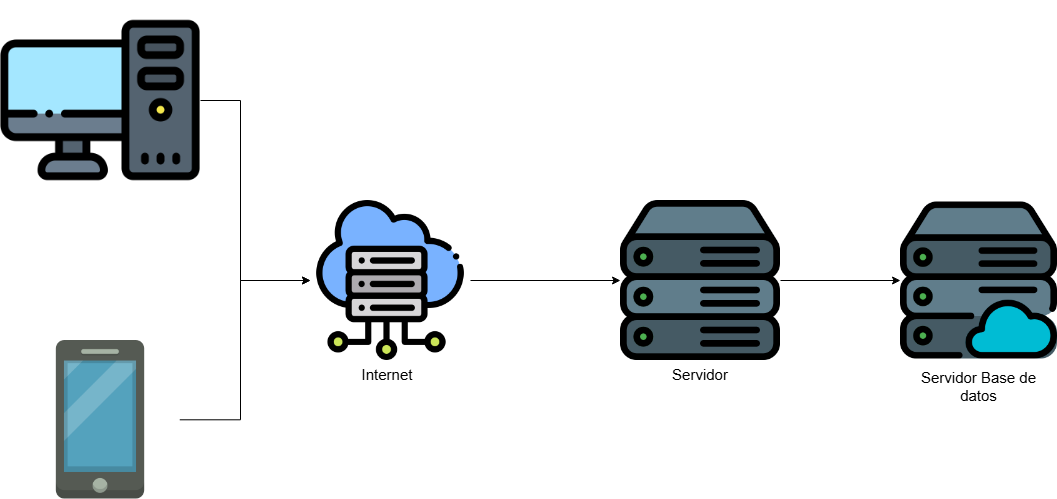
\includegraphics[bb=0 0 640 480, width=.6\linewidth]{imagenes/Diagrama fisico.drawio.png}
  \vspace*{1cm}
  \caption{Arquitectura física}
\end{figure}

\subsection{Arquitectura lógica}
La arquitectura lógica propuesta sigue el patrón Modelo-Vista-Controlador (MVC). En la figura 4.2 se ilustra la comunicación bidireccional entre sus componentes. La capa 'Vistas' se encarga de mostrar la información al usuario a través de las interfaces, según los datos recibidos de la capa 'Controladores', la cual se encarga de manejar la lógica del sistema, procesando las peticiones POST, GET, PUT y DELETE que provienen de la vista. La capa 'Modelos' se usa para gestionar la estructura de datos y las reglas del sistema, permitiendo la gestión de información. Finalmente, la capa 'Base de datos' se encarga de guardar y entregar la información correctamente.
\begin{figure}[H]
  \vspace*{1cm}
  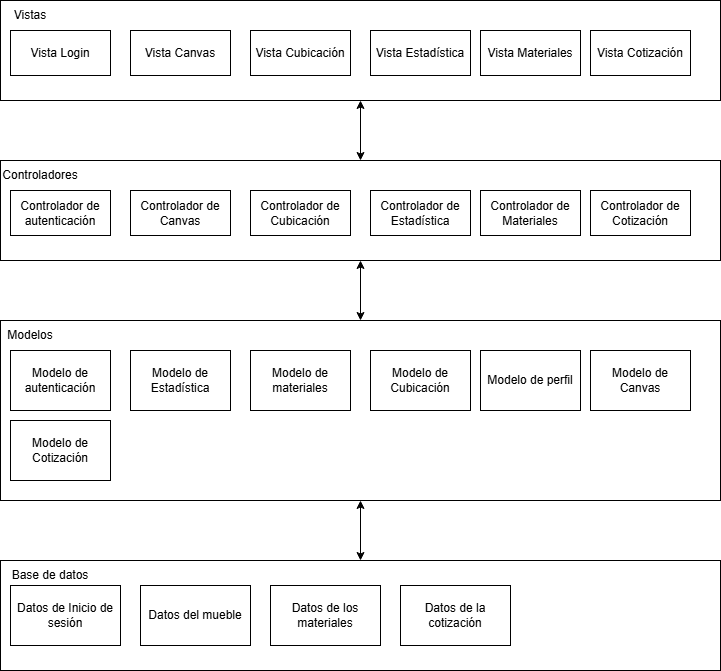
\includegraphics[ width=.9\linewidth]{imagenes/diagramaFormulacionlogico.drawio.png}
  \vspace*{1cm}
  \caption{Arquitectura lógica}
\end{figure}

\subsection{Modelo de datos}
Como se mencionó anteriormente el esquema de base de datos a utilizar no es SQL por lo que hacer un diagrama ER no es la mejor representación, por lo que mediante la herramienta 'Hackolade', que es una herramienta de modelado de datos pude representar el funcionamiento de la base de datos NoSQL de una manera más visual y familiar entiendiéndose como similar a un diagrama ER.


\begin{figure}[H]
  \vspace*{1cm}
  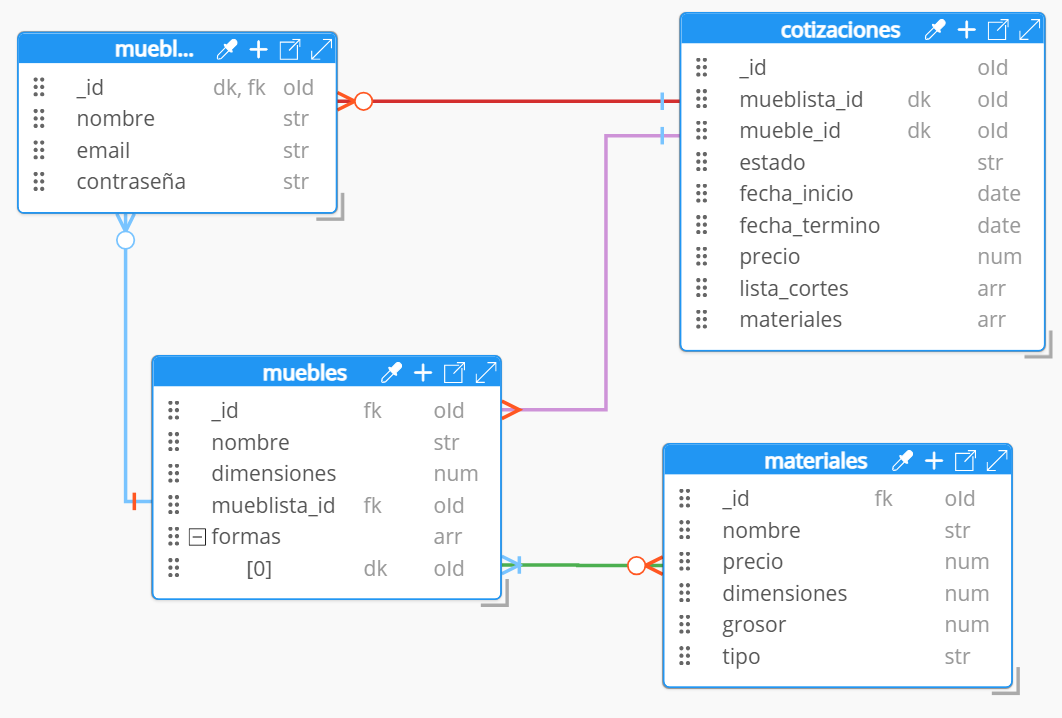
\includegraphics[width=.9\linewidth]{imagenes/modelo de datos.png}
  \vspace*{1cm}
  \caption{Modelo de datos}
\end{figure}

\subsection{Diagrama de flujo}
En la figura 4.4 se ilustra el flujo general del funcionamiento de la aplicación que es desde que inicia sesión, continuando con el diseño del mueble en donde lo modifica según los requisitos que requiera, para pasar a cubicación en donde se calcula la cantidad de material requerido y lo entrega en la vista para posteriormente pasar a la cotización en donde se hace el cálculo a partir de los precios en la base de datos. 


\begin{figure}[H]
  \vspace*{1cm}
  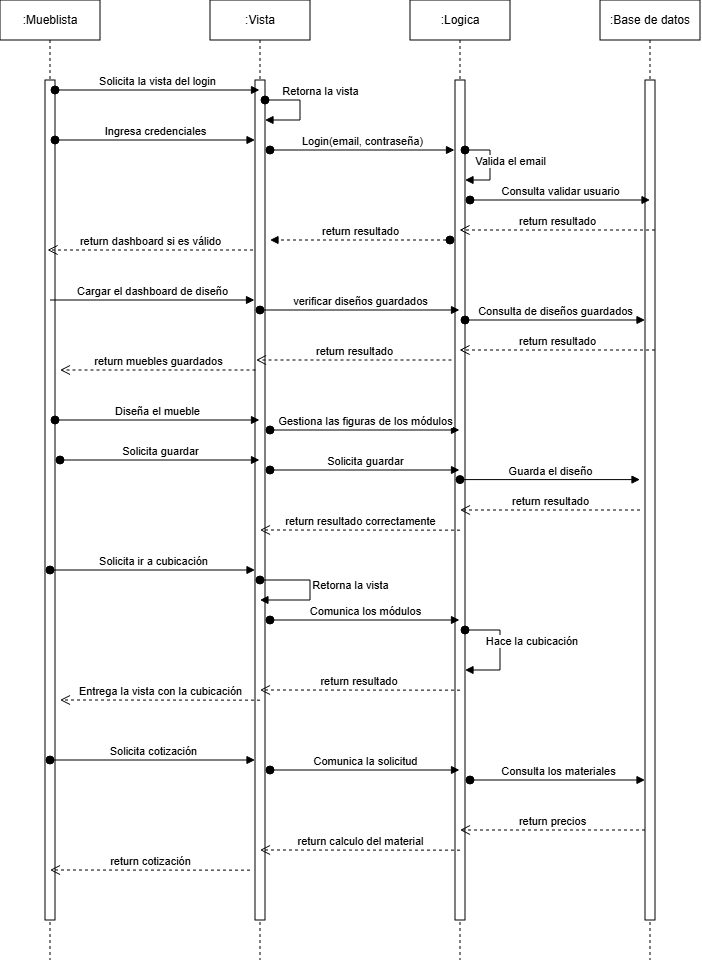
\includegraphics[width=.9\linewidth]{imagenes/general.drawio.png}
  \vspace*{1cm}
  \caption{Diagrama de secuencia}
\end{figure}

\subsection{Mockups}
En este apartado se presentan algunos de los mockups propuestos durante el proceso de desarrollo del sistema, los cuales fueron diseñados y planificados en base a los requerimientos funcionales. Estos mockups tienen como función ilustrar las principales interfaces del sistema.
\begin{figure}[H]
  \vspace*{1cm}
  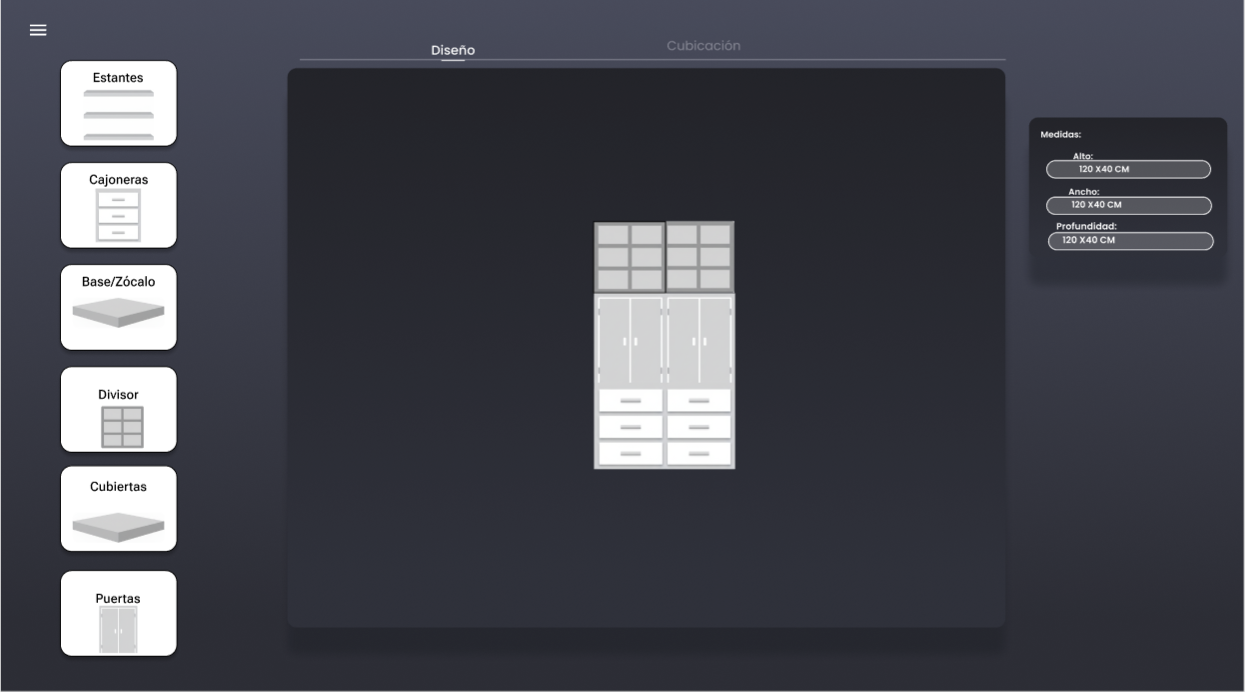
\includegraphics[bb=0 0 640 480, width=.8\linewidth]{imagenes/mockup1.png}
  \vspace*{1cm}
  \caption{Mockup dashboard de diseño canvas en dispositivo de escritorio (PC, Notebook)}
\end{figure}
La figura 4.5 ilustra la vista luego de que un usuario se autentique, donde se
presentan todos los componentes que puede interactuar dentro del sistema (siendo la vista pensada para computador).
\begin{figure}[H]
  \vspace*{1cm}
  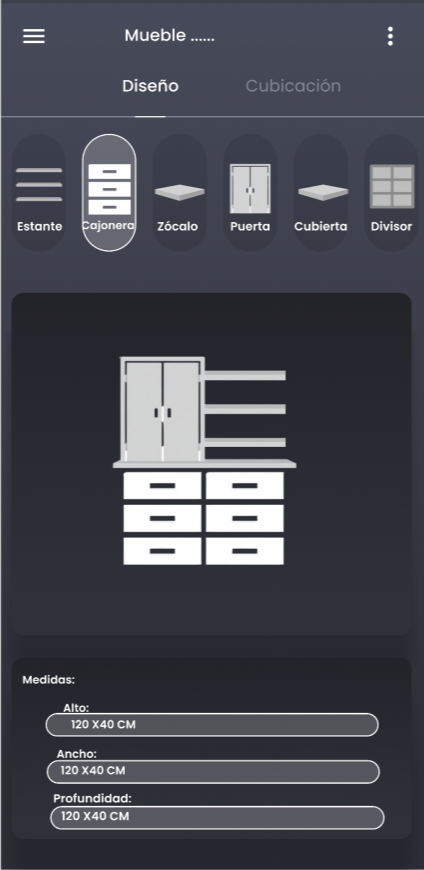
\includegraphics[bb=0 0 640 480, width=.9\linewidth]{imagenes/Mockup2.png}
  \vspace*{1cm}
  \caption{Mockup dashboard de diseño canvas en dispositivo móvil}
\end{figure}
La figura 4.6 ilustra la vista luego de que un usuario se autentique, donde se
presentan todos los componentes que puede interactuar dentro del sistema (siendo la vista pensada para teléfono celular).

\section{Iteraciones}
A continuación, se detallan como se abordaron las iteraciones descritas en el Capítulo 3.1.3

\subsection{Iteración 1}
En esta iteración la historia de usuario a trabajar es HU01: Como usuario quiero iniciar sesión en el sistema. Para esto primero tuve que configurar el entorno del proyecto, es decir, crear repositorios necesarios, descargar las técnologías necesarias para comenzar el desarorrollo. Una vez finalizada la instalación y configuración de las dependencias necesarias se da comienzo a la implementación de la metodología PXP.  

\subsubsection{Inicio de Iteración}
En esta etapa, se crean y registran las tareas acordes a las historias de usuario a trabajar, en donde en el cuadro 4.1 se ilustra las tareas resultantes para la iteración.

\begin{table}[H]
    \centering
    % --- La \caption va primero para que aparezca arriba ---
    \caption{Tareas asociadas a historias de usuario}
    \label{tab:tareas_historias_de_usuario} 
    
    % --- INICIO DE LA TABLA ---
    \begin{tabular}{|p{2cm}|p{2cm}|p{7cm}|} 
        \hline % Línea horizontal superior
        
        % Encabezados en negrita
        \textbf{HU } & \textbf{Tarea} & \textbf{Descripción}\\
        \hline % Línea de separación
        
        % --- Filas con \hline después de CADA una ---
HU01 & T01 & Crear diagrama de secuencia\\
\hline
HU01 & T02 & Crear vista para el inicio de sesión\\
\hline
HU01 & T03 & Crear ruta para inicio de sesión\\
\hline
HU01 & T04 & Creación y testeo de pruebas unitarias\\

        \hline % Línea horizontal inferior
    \end{tabular}
\end{table}

\subsubsection{Diseño}
En esta etapa, se diseña  diagrama de secuencia de la funcionalidad de la iteración. A continuación, en la figura 4.6 se ilustra el flujo del inicio de sesión 

\begin{figure}[H]
  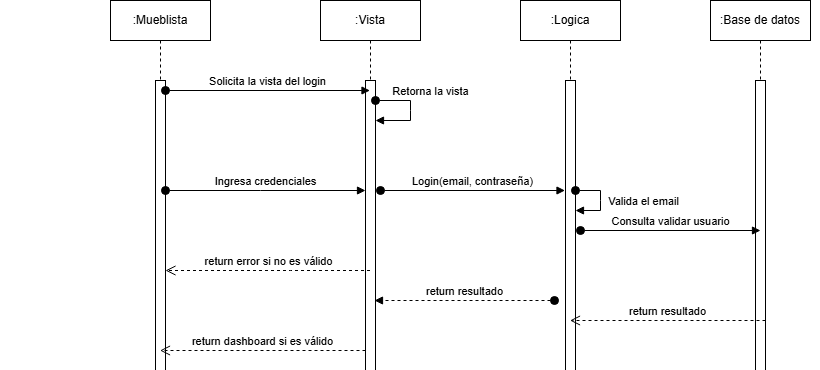
\includegraphics[width=1\linewidth]{imagenes/secuencia2.drawio.png}
  \caption{diagrama de secuencia HU01: login}
\end{figure}
\subsubsection{Implementación}
Para dar inicio a esta iteración se comienza instalando todas las dependencias y paquetes que en este caso es instalar React~\cite{react} con su adaptación a JavaScript, Konva.js~\cite{konva}, Mongoose para poder utilizar MongoDB~\cite{mongodb} y Node.js~\cite{nodejs} con express para poder hacer el backend.
Una vez realizado eso procedemos a trabajar en HU01 que es el Login, para esto primero creamos la el formulario del login.
\begin{figure}[H]
  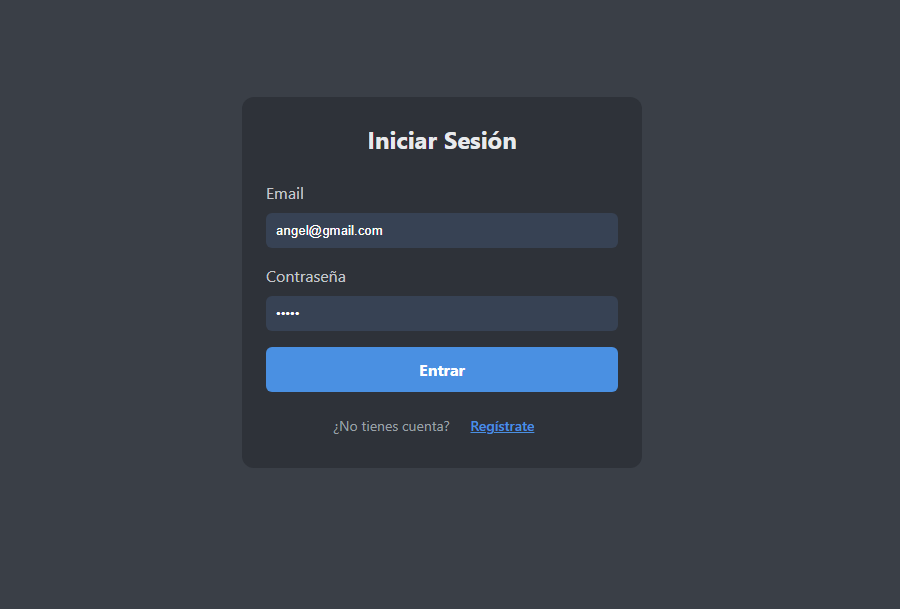
\includegraphics[width=1\linewidth]{imagenes/Screenshot_1.png}
  \caption{frontendlogin}
\end{figure}

También se tiene que crear el modelo con el cual se van a guardar los datos del mueblista para un próximo inicio de sesión.
\begin{figure}[H]
  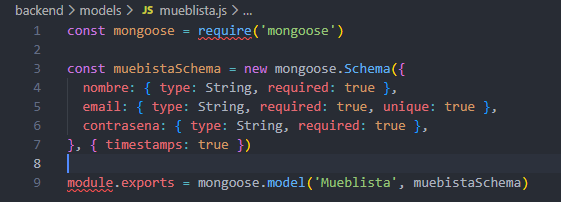
\includegraphics[width=1\linewidth]{imagenes/modelo_mueblista.png}
  \caption{modelo de datos mueblista}
\end{figure}

Una vez creado el formulario y lo que va contener la base de datos se crea la lógica para poder utilizar el formulario, en donde se crea la función de AuthForm para autenticar el formulario y tenemos la variable para identificar si esta en el formulario de registro o de login/iniciar sesión, para después validar los datos y crear el token para mantener la sesión iniciada y poder guardar y cargar los diseños de muebles.
\begin{figure}[H]
  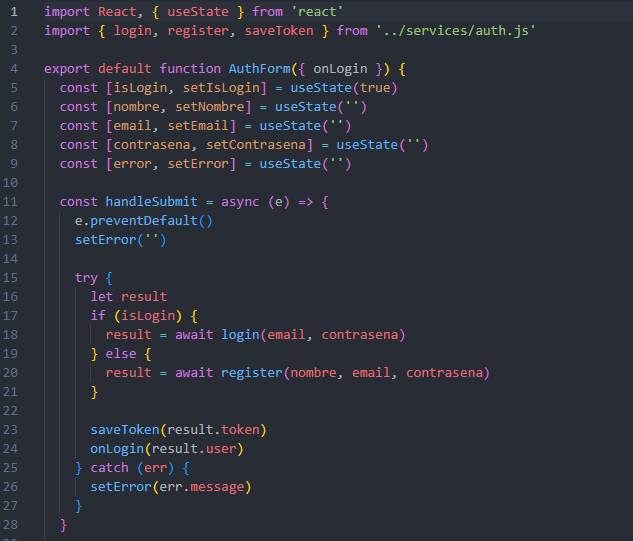
\includegraphics[width=1\linewidth]{imagenes/logica_login.png}
  \caption{Backend login}
\end{figure}
Una vez creado el Frontend, el Backend y el modelo de la base de datos procedemos a crear las rutas para poder registrar y validar credenciales. Entonces, para poder hacer registro de un nuevo usuario se llama al método 'register' al cual se le entrega el nombre, email y contraseña (la cual se cifra con bcryptjs) para ser guardado en la base de datos y se le crea un token para mantener la sesión iniciada y validar que mueblista está usando el programa, todo esto se muestra en la figura 4.11. Para el login se crea la ruta consultando con los datos email y contraseña en donde son buscados en la base de datos para encontrar si corresponden y si son correctos se crea un token para poder mantener la sesión iniciada en el navegador como se muestra en la figura 4.12. Además, se crea la verificación del token para asegurar que usuario esta conectado al programa y esta interactuando con las funcionalidades como se muestra en la figura 4.13 son solo validaciones en la cual se asegura la existencia del token y si no lo tiene se se asigna uno predeterminado.
\begin{figure}[H]
  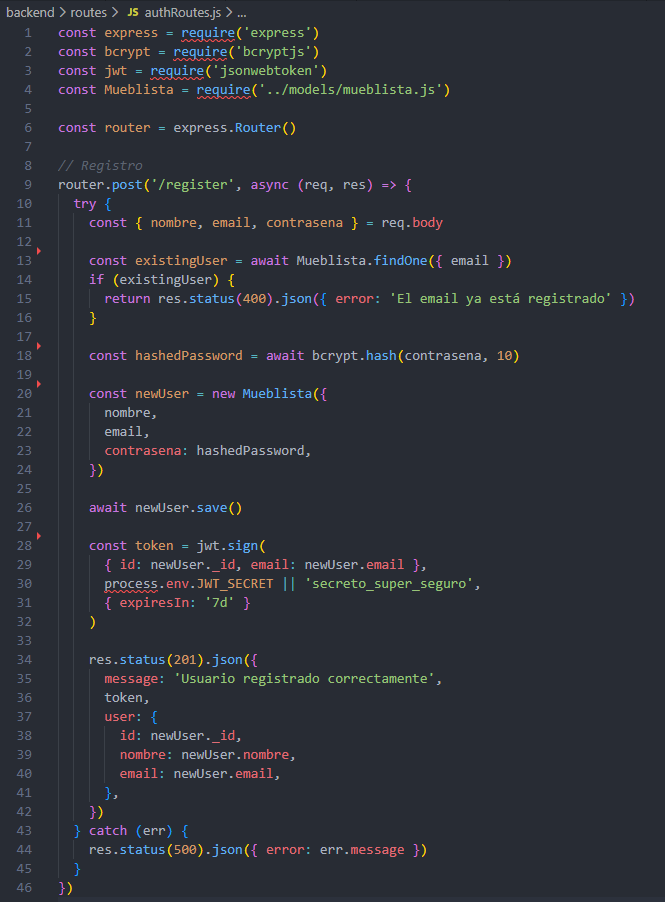
\includegraphics[width=1\linewidth]{imagenes/ruta_registro.png}
  \caption{Ruta login (registro)}
\end{figure}
\begin{figure}[H]
  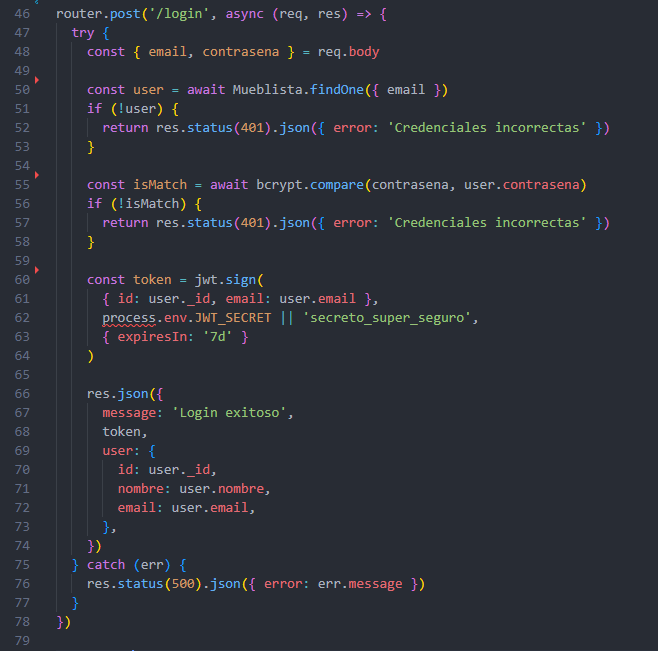
\includegraphics[width=1\linewidth]{imagenes/ruta_login.png}
  \caption{Ruta login (validación)}
\end{figure}
\begin{figure}[H]
  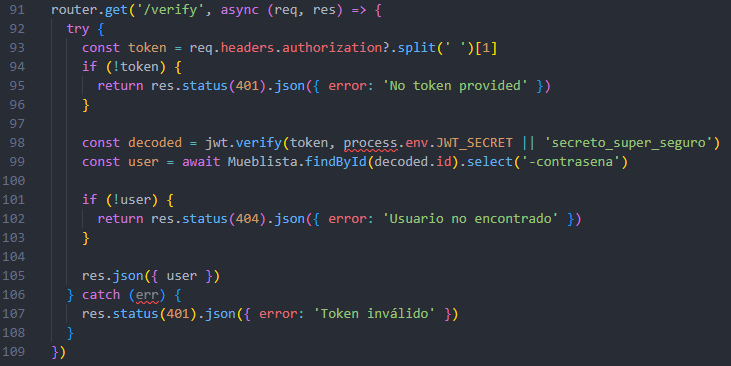
\includegraphics[width=1\linewidth]{imagenes/ruta_jwt.png}
  \caption{Ruta login (verificación token)}
\end{figure}
\subsubsection{Sistema de pruebas}
Después de la implementación, se continua con las pruebas de la iteración en donde se evaluan los siguientes casos:
\begin{itemize}
    \item Ingresar credenciales válidas.
    \item Ingresar credenciales inválidas.
    \item Ingresar una dirección de correo incompleta.
\end{itemize}

\subsubsection{Retrospectiva}
Al final esta iteración, se revisa el peso asignado a las historias de usuario, en esta iteración fue acertada y se completó la funcionalidad sin pendientes.

\subsection{Iteración 2}
En esta iteración la historia de usuario a trabajar es HU02: Como ususario quiero un canvas 2D para poder hacer diseños, HU03: Como usuario quiero crear, guardar, cargar y eliminar el diseño de un mueble, HU04: Como usuario quiero que el diseño se pueda hacer módular, HU05: Como usuario quiero que las medidas de los módulos agregados puedan ser editables, HU06: Como usuario quiero que los módulos sean móviles para acomodarlos según la necesidad. Para esto da comienzo a la implementación de la metodología PXP.  

\subsubsection{Inicio de Iteración}
En esta etapa, se crean y registran las tareas acordes a las historias de usuario a trabajar, en donde en el cuadro 4.2 se ilustra las tareas resultantes para la iteración.

\begin{table}[H]
    \centering
    % --- La \caption va primero para que aparezca arriba ---
    \caption{Tareas asociadas a historias de usuario}
    \label{tab:tareas_historias_de_usuario} 
    
    % --- INICIO DE LA TABLA ---
    \begin{tabular}{|p{2cm}|p{2cm}|p{7cm}|} 
        \hline % Línea horizontal superior
        
        % Encabezados en negrita
        \textbf{HU } & \textbf{Tarea} & \textbf{Descripción}\\
        \hline % Línea de separación
        
        % --- Filas con \hline después de CADA una ---
HU02, HU03, HU04, HU05, HU6 & T01 & Crear diagrama de secuencia\\
\hline
HU02 & T02 & Crear canvas 2D\\
\hline
HU02 & T03 & Crear ruta para el canvas\\
\hline
HU02 & T04 & Crear figuras para el canvas\\
\hline
HU03 & T05 & Crear botones de Crear, guardar, cargar y eliminar\\
\hline
HU03 & T06 & Crear rutas para los botones\\
\hline
HU04 & T07 & Modificar las propiedades de las figuras \\
\hline
HU05 & T08 & Creación de etiquetas para ingresar medidas\\
\hline
HU05 & T09 & Creación rutas para el ingreso de medidas \\
\hline
HU06 & T010 & Modificar las propiedades de las figuras\\
\hline
HU02, HU03, HU04, HU05, HU6 & T011 & Creación y testeo de pruebas unitarias\\
        \hline % Línea horizontal inferior
    \end{tabular}
\end{table}

\subsubsection{Diseño}
En esta etapa, se diseña  diagrama de secuencia de la funcionalidad de la iteración. A continuación, en la figura 4.7 se ilustra el flujo del inicio de sesión 

\begin{figure}[H]
  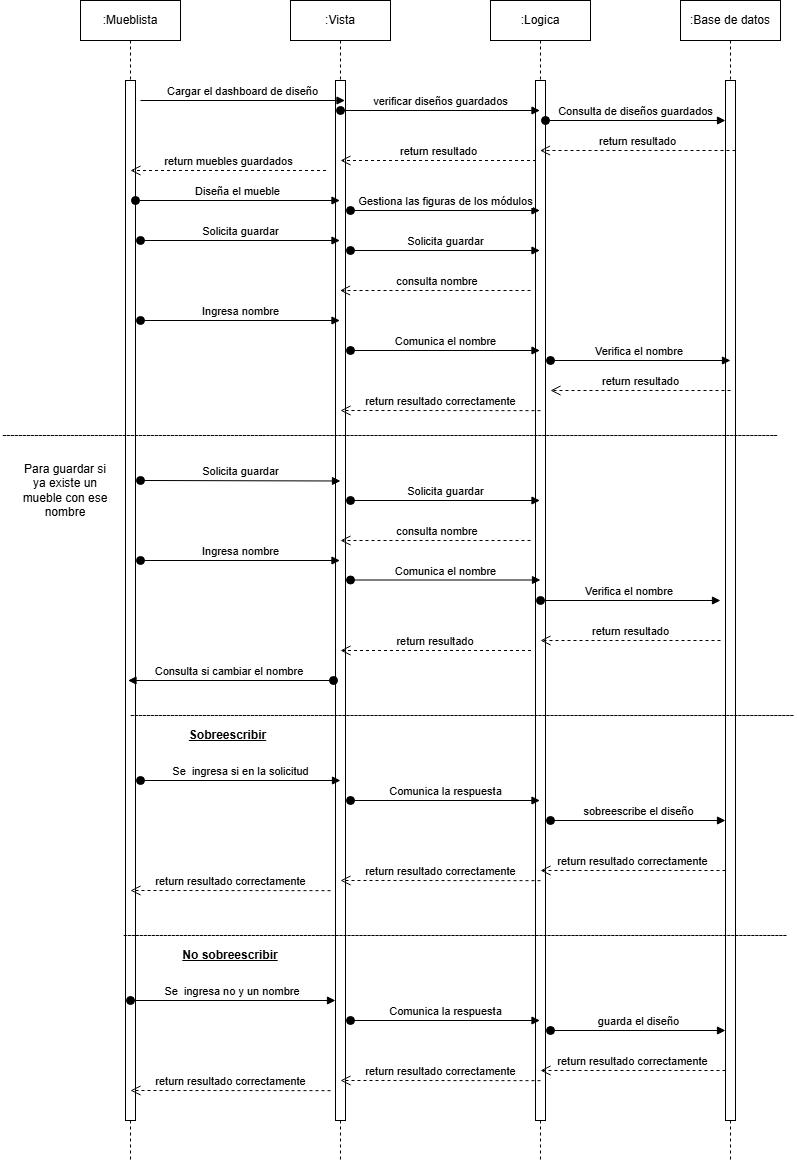
\includegraphics[width=1\linewidth]{imagenes/canvas.drawio.png}
  \caption{diagrama de secuencia HU02, HU03, HU04, HU05, HU6: Canvas}
\end{figure}
\subsubsection{Implementación}

En la figura 4.15 se muestra la función encargada de guardar los diseños de los muebles con sus correspondientes atributos en donde se guarda en un array las formas Creadas en el canvas.
\begin{figure}[H]
  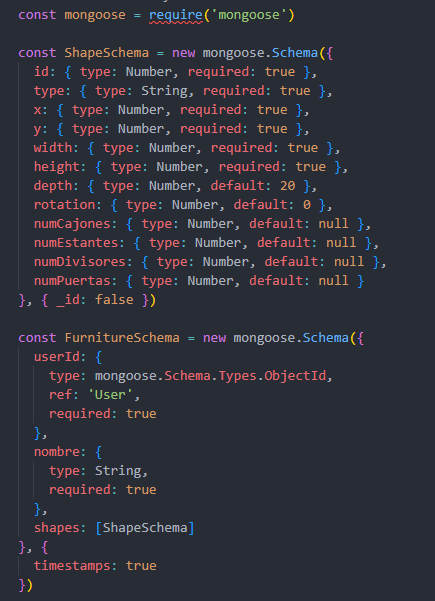
\includegraphics[width=.8\linewidth]{imagenes/furnitures.png}
  \caption{Guardado de diseños}
\end{figure}
En la figura 4.16 se muestra las instancias de creación de cada forma para crear los módulos de los muebles en donde las medidas son en centímetros y cada figura cuenta con ancho, alto y profundidad (No se ilustra la profundidad ya que sirve para el futuro cálculo de material)
\begin{figure}[H]
  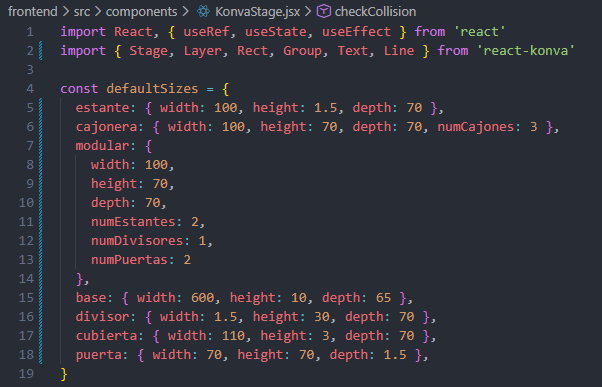
\includegraphics[width=1\linewidth]{imagenes/creacion_partes.png}
  \caption{Inicialización de figuras}
\end{figure}

En la figura 4.17 se muestra el funcionamiento del módulo de cajonera en donde pide el número de cajones para que el mueblista no tenga que hacer cada cajón, en donde se tiene por predefinido 3 cajones y si se quiere cambiar se hace la división de la altura entre la cantidad de cajones para dividir cómodamente el espacio. 
\begin{figure}[H]
  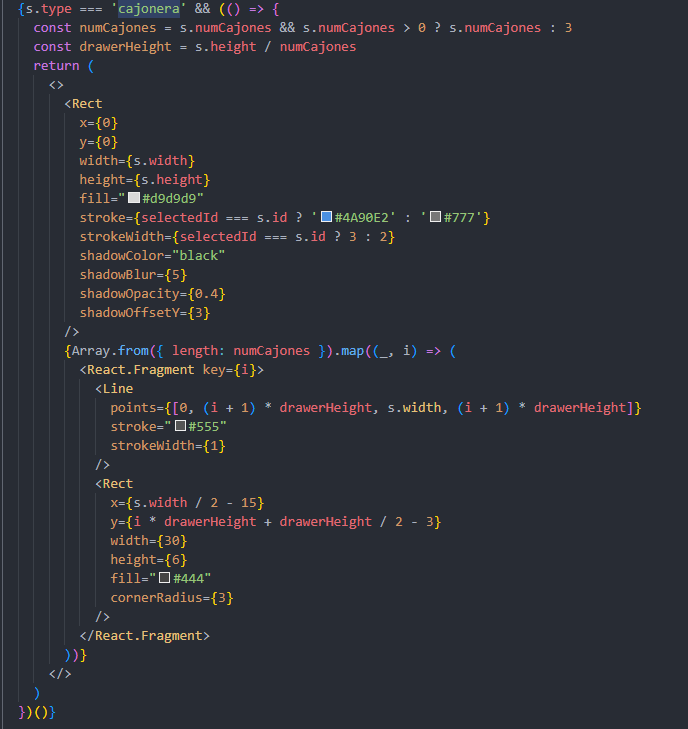
\includegraphics[width=1\linewidth]{imagenes/cajonera.png}
  \caption{Módulo de cajonera}
\end{figure}

En la figura 4.18 y 4.19 se muestra la lógica detrás del fuincionamiento del módulo modular que es una figura que contiene el cubo de la figura, cantidad ajustable de estantes, divisores y puertas según se requiera, en donde funciona de la misma manera que en la cajonera se cálcula el alto entre estantes se requieran, el ancho entre divisores y el ancho entre las puertas para así dividir el módulo y ser uno de las figuras más completas y necesarias para hacer el diseño de un mueble. 
\begin{figure}[H]
  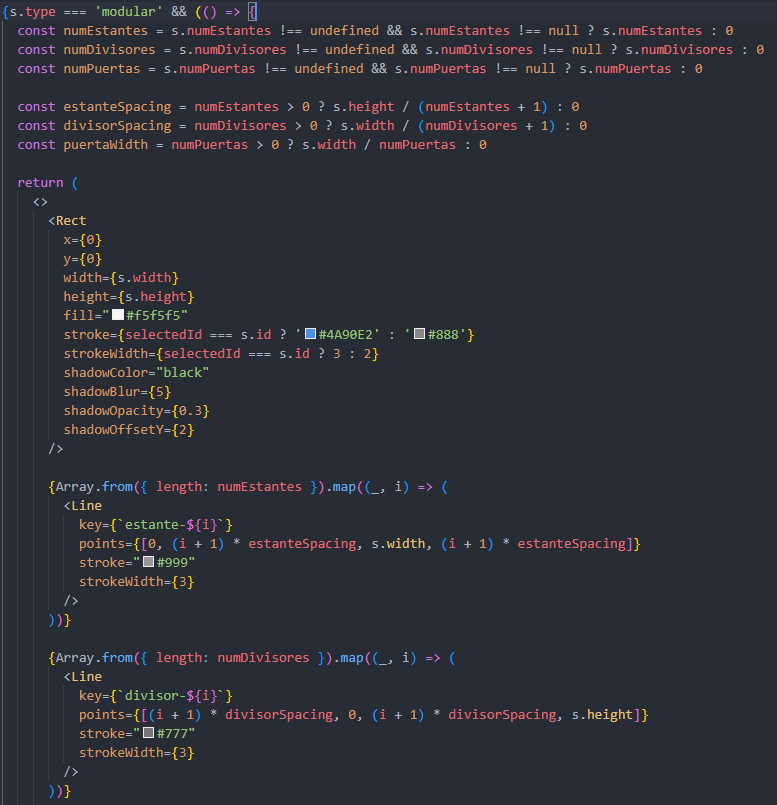
\includegraphics[width=1\linewidth]{imagenes/modular1.png}
  \caption{Módulo principal}
\end{figure}
\begin{figure}[H]
  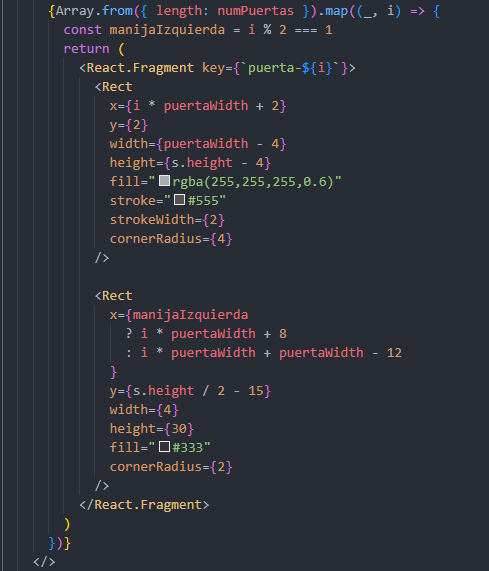
\includegraphics[width=1\linewidth]{imagenes/modular2.png}
  \caption{Módulo principal puertas}
\end{figure}

En la figura 4.20 se muestra la función encargada de guardar los diseños de muebles en la cual se valida el 'id' del mueblista y el nombre del diseño, para recopilar los atributos del diseño y ser guardados en la base de datos y ser accesible en una próxima instancia.
\begin{figure}[H]
  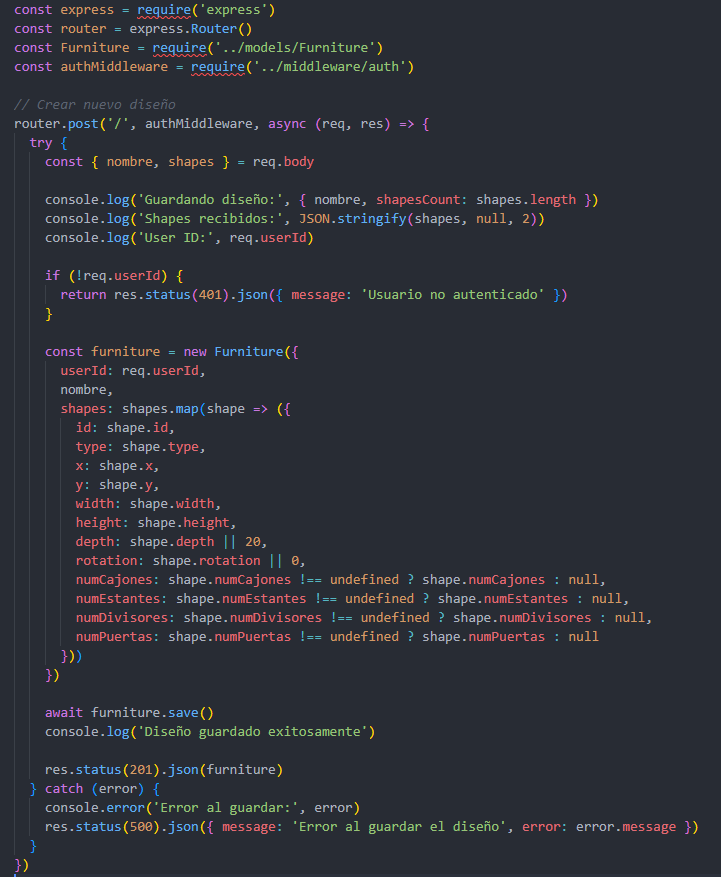
\includegraphics[width=1\linewidth]{imagenes/rutaguardar.png}
  \caption{Ruta para guardar diseños de muebles}
\end{figure}

En la figura 4.21 se encarga de obtener todos los diseños de muebles que haya guardado el mueblista, esta función recopila según el 'id' y los carga para ser mostrados en un apartado del front.
\begin{figure}[H]
  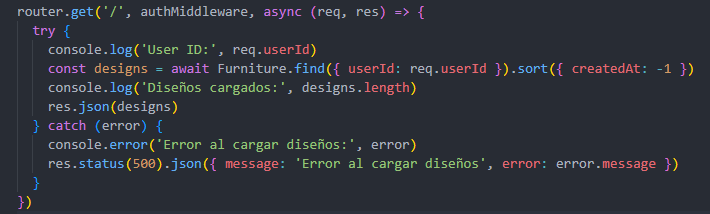
\includegraphics[width=1\linewidth]{imagenes/rutacargar.png}
  \caption{Ruta para cargar diseños de muebles}
\end{figure}

En la figura 4.22 se encarga eliminar el diseño de mueble selecionado mediante la solicitud delete, a lo cual se valida la existencia del diseño para poder ser eliminado.
\begin{figure}[H]
  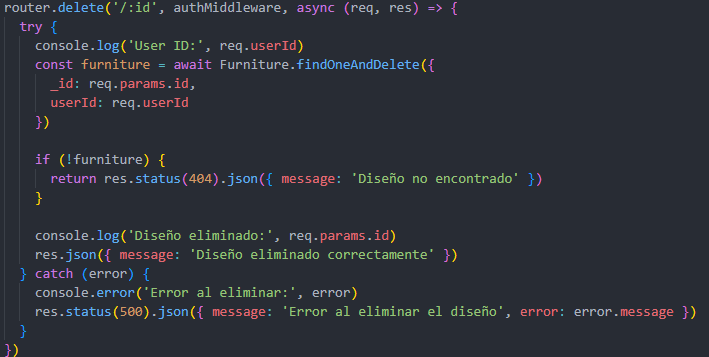
\includegraphics[width=1\linewidth]{imagenes/rutaeliminar.png}
  \caption{Ruta para eliminar diseños de muebles}
\end{figure}

En la figura 4.23 se muestra la función encargada de la actualización de diseños en donde se obtienen cuando se quiere sobreescribir desde el Frontend. Se basa en recopilar todos los datos del diseño y buscar el diseño con el mismo nombre para actualizarlo o sobreescribirlo.
\begin{figure}[H]
  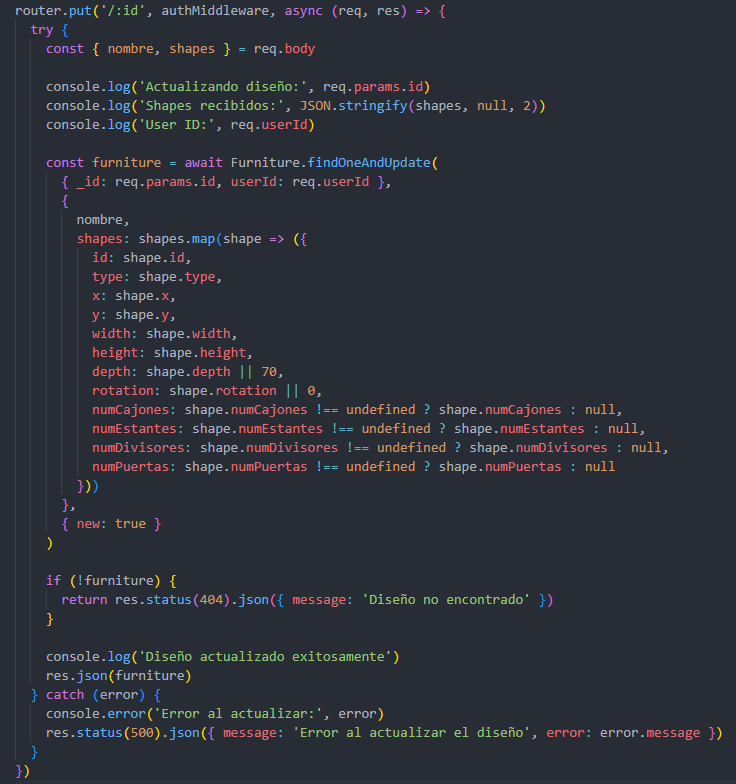
\includegraphics[width=1\linewidth]{imagenes/rutaactualizar.png}
  \caption{Ruta para actualizar diseños de muebles}
\end{figure}




\subsubsection{Sistema de pruebas}
Después de la implementación, se continua con las pruebas de la iteración en donde se evaluan los siguientes casos:
\begin{itemize}
    \item Crear figuras.
    \item Mover figuras.
    \item Editar medidas de las figuras.
    \item Guardar diseños de muebles.
    \item Cargar diseños de muebles.
    \item Eliminar diseños de figuras.
    \item Eliminar diseños de muebles.
    \item Guardar diseños de muebles con el mismo nombre.
\end{itemize}

\subsubsection{Retrospectiva}
Al final esta iteración, se revisa el peso asignado a las historias de usuario, en esta iteración fue subestimado y no se ha terminado completamente la iteración.

\chapter{Conclusiones y trabajo futuro}
En este capítulo se abarcan las conclusiones obtenidas del trabajo realizado y de lo que queda por realizar en el proyecto.
\section{Cumplimiento de Objetivos}
Dado que el desarrollo actualmente está en la iteración 2, la cual está relacionada con el Objetivo Específico 1: Implementar una aplicación web que provea de un espacio de diseño en dos dimensiones (2D) orientado a muebles para que el fabricante pueda generar diseños personalizados en base a los requisitos del cliente. Entonces, como se menciona en el capítulo 4.3.2 ya está desarrollado lo principal que es el espacio de diseño, solo falta mejorar el espacio de diseño como por ejemplo que la colisión no funcione igual para una puerta como para una cubierta.\\


Hasta el momento se cuenta con este resultado en la encuesta SUS\\
1. Creo que me gustaría utilizar este sistema con frecuencia.= 5\\
2. Encontré el sistema innecesariamente complejo = 2\\
3. Pensé que el sistema era fácil de usar = 4\\
4. Creo que necesitaría el apoyo de un técnico para poder utilizar este sistema = 1\\
5. Encontré que las diversas funciones de este sistema estaban bien integradas = 3\\
6. Pensé que había demasiada inconsistencia en este sistema = 1\\
7. Me imagino que la mayoría de la gente aprendería a utilizar este sistema muy rápidamente = 5\\
8. Encontré el sistema muy complicado de usar = 1\\
9. Me sentí muy seguro usando el sistema = 4\\
10. Necesitaba aprender muchas cosas antes de empezar con este sistema = 2\\

Suma: 4 + 3 + 3 + 4 + 2 + 4 + 4 + 4 + 3 + 3 = 34\\

Puntaje SUS: 34 × 2.5 = 85\\
\section{Reflexión Final del Proyecto}
Esta propuesta está siendo un desafío que pone a prueba lo aprendido durante el desarrollo de la carrera, desde el momento del planteamiento del problema, el como solucionarlo y el método para soluicionarlo, además de toda la aplicación de conocimientos técnicos que van de la mano con el desarrollo.


\section{Trabajo Futuro}
Como trabajo futuro me queda:
\begin{itemize}
    \item Mejorar los íconos de la interfaz.
    \item Mejorar la colisión de las figuras.
    \item Indagar sobre un algoritmo para la cubicación.
    \item Desarrollar en los módulos de materiales.
    \item Desarrollar en los módulos de cotizaciones.
    \item Desarrollar en los módulos de cubicación.
    \item Desarrollar en los módulos de estadística.
    \item Implementar el método para que el usuario/mueblista pueda recuperar su contraseña.
\end{itemize}

\bibliography{refs}



\appendixpart
\appendix{Carta Gantt}
\begin{figure}[H]
  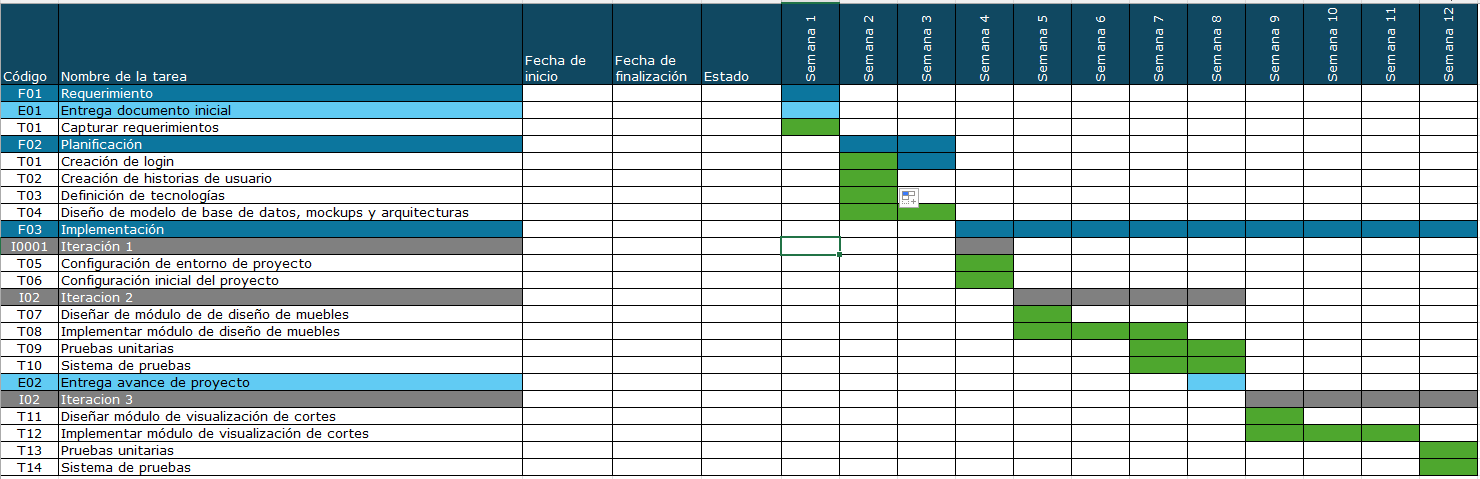
\includegraphics[width=1\linewidth]{imagenes/carta.png}
  \caption{carta Gantt}
\end{figure}
\begin{figure}[H]
  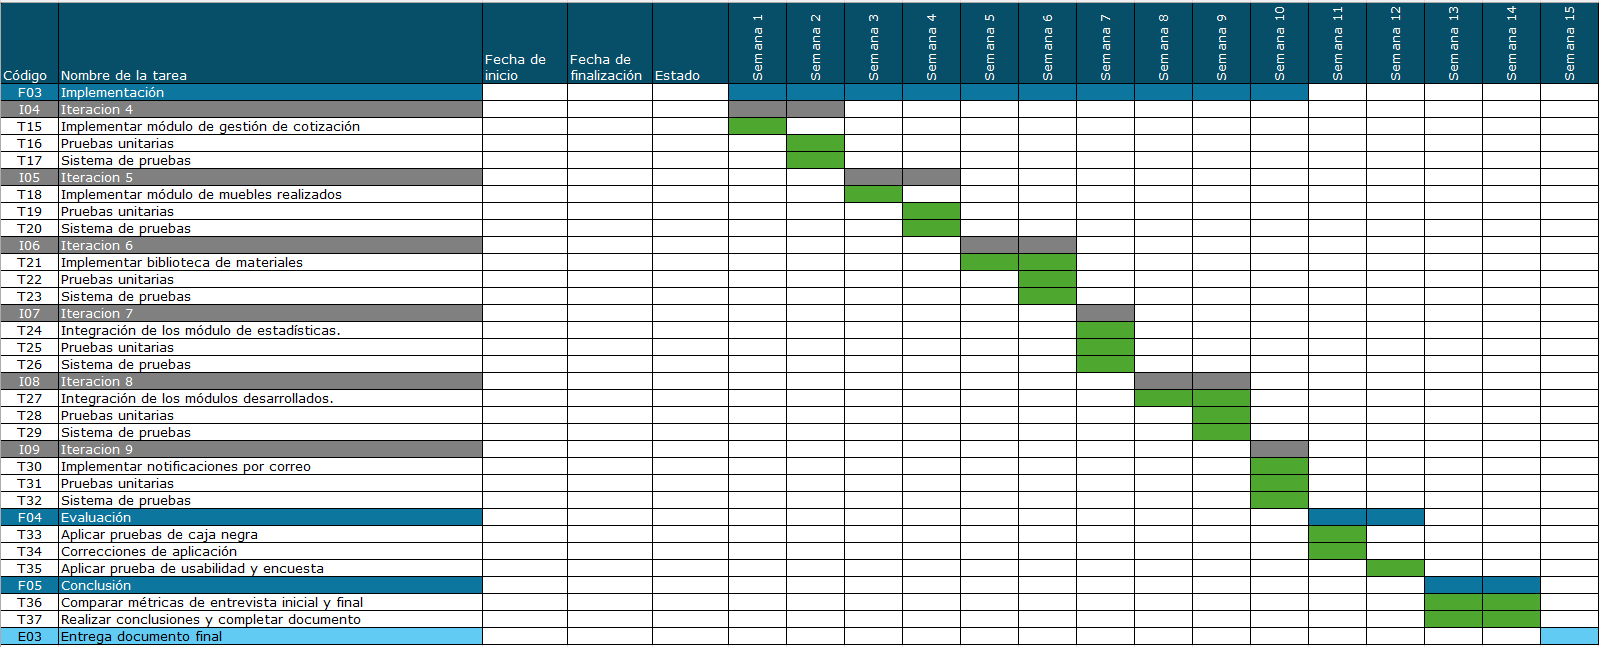
\includegraphics[width=1\linewidth]{imagenes/gantt.png}
  \caption{carta Gantt}
\end{figure}

%% fin
\end{document}
